\documentclass[anon]{alt2027}
\usepackage{times}
\setcitestyle{round}
\usepackage[T1]{fontenc}
\usepackage{mathtools}
\usepackage{placeins}
\usepackage{booktabs}
\usepackage{tikz}
\usepackage{comment}
\usetikzlibrary{decorations.pathreplacing,arrows.meta}
\usepackage{enumitem}
\usepackage[expansion=false]{microtype}
\hypersetup{colorlinks,linkcolor=blue!60!black,citecolor=blue!60!black,urlcolor=blue!60!black}

\newcommand{\PORT}[1]{{\color{red}[\textbf{PORT:} #1]}}
\newcommand{\price}{\rho}
\newcommand{\rate}{I}
\newcommand{\op}{\omega}
\newcommand{\Mlab}{M_{\mathrm{lab}}}
\newcommand{\batchreg}{R^{\mathrm{B}}}
\newcommand{\Xd}{\mathcal{X}_d}
\newcommand{\simplex}{\Delta_d}
\newcommand{\LSA}{\mathcal{M}_{d,L}}
\newcommand{\Exp}{\operatorname{Exp}}
\newcommand{\Dir}{\operatorname{Dirichlet}}
\newcommand{\Mult}{\operatorname{Multinomial}}
\newcommand{\profile}{\operatorname{profile}}
\newcommand{\E}{\mathbb{E}}
\newcommand{\Prob}{\mathbb{P}}
\newcommand{\cstar}{c^{\star}}
\newcommand{\Lmax}{L_{\max}}
\newcommand{\KL}{\operatorname{D}}
\renewcommand{\eqref}[1]{(\ref{#1})}

% Keep the JMLR last-page label without a trailing empty box that can create a blank page.
\makeatletter
\patchcmd{\@jmlrenddoc}{\label{jmlrend}\null}{\label{jmlrend}}{}{}
\makeatother

\title[A Layered Simplex Architecture]{A Layered Simplex Architecture for Large Alphabets}
\altauthor{\Name{Anonymous authors}}

\begin{document}
\maketitle

\begin{abstract}
Estimating a distribution over a large alphabet is hard when the sample is smaller than the alphabet and most symbols are rarely observed. We take a Bayesian approach and study a model in which the depth of an architecture shapes the prior: the \emph{layered simplex architecture} multiplies $L$ independent uniformly distributed points of the simplex coordinate-wise and normalizes. At depth one its predictor is Laplace's rule; greater depth moves prior mass toward concentrated distributions. We derive an exact one-dimensional representation of the marginal likelihood, computed successively across depths, and count-profile expressions for the regret; a further mixture averages over depths while reusing the kernel computations. We prove that every label-invariant predictor pays at least the expected description length of the discovered symbols minus the conditional entropy of their identities given their number, and that for Zipf targets with $\alpha>1$ and $d=N^{\nu+o(1)}$, $\nu>1/\alpha$, the depth mixture attains this to leading order: the regret exponent $1-1/\alpha$ is determined by the rate of symbol discovery. Experiments on synthetic sources and the King James Bible show large gains over add-constant rules on concentrated targets and competitive performance with Good--Turing and Ristad's law. The architecture extends naturally to layers raised to powers, with a Bayesian mixture over the exponents. The layered simplex architecture provides a simple, analytically accessible instance of the recently proposed view that an architecture induces a prior with a broad complexity spectrum.
\end{abstract}

\section{Introduction}
\label{sec:intro}

Estimating a distribution on a $d$-symbol alphabet from $N$ samples under log loss is easier when $N\gg d$, and harder when the alphabet is large relative to the data. Classical Bayesian rules such as Laplace's add-one rule and the Krichevsky--Trofimov add-half rule~\citep{krichevsky1981performance} spread probability over the whole alphabet. They can therefore perform poorly when the target distribution is concentrated. Good--Turing estimators~\citep{good1953population} are designed for this regime and have strong theoretical guarantees~\citep{orlitsky2003always,mcallester2000leave,acharya2013tight,orlitsky2015competitive}. Ristad's law~\citep{ristad1995natural} shows that a hierarchical Bayesian model can recover some of the same ability to adapt. Our central contribution is the combination of a simple multiplicative construction, explicit analytic expressions for its evidence and regret, and broad empirical competitiveness. These expressions make the connection between the architecture and its performance accessible to both mathematical analysis and numerical evaluation. This paper asks three questions:

\paragraph{Can a simple Bayesian prior compete in the large-alphabet regime?}
Multiplying independent random probability assignments still treats all labels in the same way. The number of layers controls how concentrated the resulting prior is. We study this \emph{layered simplex architecture} (LSA; Figure~\ref{fig:lsa}): draw $L$ independent uniform points $U^{(1)},\dots,U^{(L)}$ of the simplex $\simplex$, multiply them coordinate-wise, and renormalize,
\begin{equation}
\label{eq:lsa}
\theta_i \;=\; \frac{\prod_{\ell=1}^{L}U^{(\ell)}_i}{\sum_{j=1}^{d}\prod_{\ell=1}^{L}U^{(\ell)}_j},\qquad i=1,\dots,d.
\end{equation}
In Hinton's terminology~\citep{Hinton1999ProductsOE}, this construction is a random product of experts, with each $U^{(\ell)}$ acting as one expert. 
Depth---the number of layers---changes the prior distribution over a fixed model class. At every positive finite depth, the prior assigns positive probability to every open region of the simplex. The predictor is the exact Bayesian mixture $Q^{(L)}_N$ of multinomial sources under this prior. At $L=0$ the empty product gives $1$ for each component, thus  $\theta_i=1/d$ and $Q_N^{(0)}(x^N)=d^{-N}$. At $L=1$, the predictor is Laplace's rule. As depth increases, the prior favors distributions in which a few symbols carry most of the probability. The relevant depth scale grows logarithmically with $d$. For fixed $d$, the prior concentrates on the simplex vertices as $L\to\infty$. Since different depths suit different targets, we also study the depth-averaged predictor
\begin{equation}
\label{eq:avg}
Q^{\mathrm{avg}}_N(x^N)\;=\;\frac{1}{\Lmax+1}\sum_{L=0}^{\Lmax}Q^{(L)}_N(x^N),
\end{equation}
This gives a single Bayesian predictor whose set of depths is fixed before the data are observed. 

\paragraph{Can the scaling laws of such an estimator be understood from first principles?}
Empirical scaling laws describe power-law improvements with data~\citep{kaplan2020scaling}. For Zipf sources with fixed $\alpha>1$ and $d/N^{1/\alpha}\to\infty$, the expected number of distinct symbols grows as $N^{1/\alpha}$. Symbol discovery has long helped explain learning curves~\citep{hutter2021learning,michaud2023quantization,bahri2024explaining,debowski2025zipf}. Here we derive a sharp regret law for an explicit Bayesian prior.

\paragraph{What does a layered architecture buy?}
An architecture and its random initialization induce a \emph{prior over predictors}~\citep{MerhavFeder1998,feder2025framework}. Bayesian regret depends on the prior mass near the target (Section~\ref{sec:setting}). Multiplication spreads random weights over many orders of magnitude; LSA makes the resulting relation between prior and regret analytically accessible.

\begin{figure}[htp]
\centering
\resizebox{\columnwidth}{!}{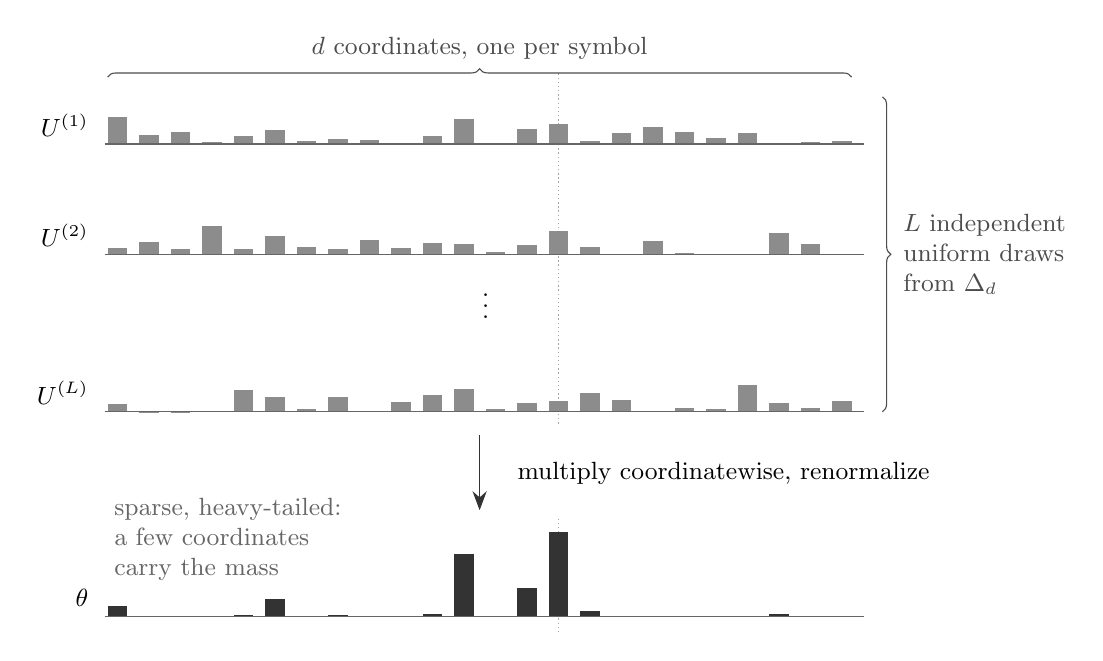
\begin{tikzpicture}[x=4.0mm,y=1mm]
  % dotted guide through the winning coordinate (drawn in two segments)
  \draw[black!35,densely dotted,line width=0.5pt] (15.31,8.5) -- (15.31,53);
  \draw[black!35,densely dotted,line width=0.5pt] (15.31,-18) -- (15.31,-3.5);
  % --- layer rows ---
  \foreach \i/\h in {1/3.43,2/1.21,3/1.53,4/0.21,5/1.02,6/1.72,7/0.35,8/0.65,9/0.53,10/0.19,11/0.99,12/3.15,13/0.07,14/1.94,15/2.54,16/0.40,17/1.39,18/2.11,19/1.47,20/0.78,21/1.44,22/0.14,23/0.30,24/0.43} \fill[black!45] (\i,44) rectangle ++(0.62,\h);
  \draw[black!60,line width=0.4pt] (0.9,44) -- (25.0,44);
  \node[left,font=\small] at (0.7,46.4) {$U^{(1)}$};
  \foreach \i/\h in {1/0.86,2/1.58,3/0.63,4/3.58,5/0.63,6/2.27,7/0.98,8/0.65,9/1.81,10/0.77,11/1.44,12/1.33,13/0.23,14/1.22,15/2.95,16/0.94,17/0.03,18/1.63,19/0.21,20/0.02,21/0.07,22/2.73,23/1.34,24/0.08} \fill[black!45] (\i,30) rectangle ++(0.62,\h);
  \draw[black!60,line width=0.4pt] (0.9,30) -- (25.0,30);
  \node[left,font=\small] at (0.7,32.4) {$U^{(2)}$};
  \node[font=\small] at (13,24.5) {$\vdots$};
  \foreach \i/\h in {1/0.99,2/0.02,3/0.02,4/0.04,5/2.73,6/1.85,7/0.30,8/1.82,9/0.12,10/1.20,11/2.09,12/2.84,13/0.30,14/1.08,15/1.39,16/2.40,17/1.46,18/0.09,19/0.45,20/0.41,21/3.37,22/1.14,23/0.54,24/1.35} \fill[black!45] (\i,10) rectangle ++(0.62,\h);
  \draw[black!60,line width=0.4pt] (0.9,10) -- (25.0,10);
  \node[left,font=\small] at (0.7,12.4) {$U^{(L)}$};
  % --- braces ---
  \draw[decorate,decoration={brace,amplitude=3pt},black!70]
    (1.0,52.5) -- (24.62,52.5) node[midway,above=3pt,font=\small] {$d$ coordinates, one per symbol};
  \draw[decorate,decoration={brace,amplitude=3pt},black!70]
    (25.6,50) -- (25.6,10) node[midway,right=4pt,align=left,font=\small]
    {$L$ independent\\ uniform draws\\ from $\Delta_d$};
  % --- arrow + operation ---
  \draw[-{Stealth[length=2.4mm]},black!80] (12.81,7) -- (12.81,-2.5);
  \node[right=8pt,align=left,font=\small] at (13.0,2.2)
    {multiply coordinatewise, renormalize};
  % --- theta row ---
  \foreach \i/\h in {1/1.31,2/0.01,3/0.02,4/0.01,5/0.21,6/2.18,7/0.03,8/0.13,9/0.02,10/0.06,11/0.35,12/7.97,13/0.00,14/3.68,15/10.72,16/0.75,17/0.01,18/0.05,19/0.03,20/0.01,21/0.02,22/0.26,23/0.11,24/0.06} \fill[black!80] (\i,-16) rectangle ++(0.62,\h);
  \draw[black!60,line width=0.4pt] (0.9,-16) -- (25.0,-16);
  \node[left,font=\small] at (0.7,-13.6) {$\theta$};
  \node[right,black!60,font=\small,align=left] at (0.9,-6.2)
    {sparse, heavy-tailed:\\ a few coordinates \\ carry the mass};
\end{tikzpicture}
}
\caption{The layered simplex architecture at $d=24$, $L=4$ (a real draw). Each layer $U^{(\ell)}$ is an independent uniform point of the simplex; their coordinate-wise product, renormalized, is the draw $\theta$ from $\LSA$, whose mass concentrates on a few coordinates. The dotted line marks the largest coordinate of $\theta$.}
\label{fig:lsa}
\end{figure}

\paragraph{Contributions.}
\begin{enumerate}[leftmargin=*,itemsep=1pt,topsep=2pt]
\item \textbf{Exact performance expressions} (Section~\ref{sec:regret}). The evidence reduces to a one-dimensional integral and the regret to count-profile expressions. Kernels are reused across depths, and we give bounds that propagate kernel and integration errors.
\item \textbf{Depth shapes the prior} (Section~\ref{sec:depth}). 
For fixed small $L$, most coordinates receive non-negligible probability. 
As $L$ grows, the prior becomes more skewed. 
For fixed $d$, the prior converges as $L\to\infty$ to a uniform mixture over the simplex vertices.
The large-deviation calculation in Appendix~\ref{app:fixedd} motivates the scaling $L=c\ln d$. 
\item \textbf{A sharp leading-order regret law} (Section~\ref{sec:scaling}). Every predictor that treats symbol labels in the same way pays at least the expected number of bits needed to identify the observed symbols, minus the source's uncertainty about their identities given their number. For Zipf sources with $\alpha>1$ and $d=N^{\nu+o(1)}$, where $\nu>1/\alpha$, the number of observed symbols grows like $N^{1/\alpha}$.
This yields per-symbol regret of order $N^{1/\alpha-1}\log N$.
\item \textbf{Empirical evidence} (Section~\ref{sec:experiments}). The depth average is competitive with Good--Turing and an adaptive Dirichlet estimator, with large gains over add-constant rules on concentrated targets (Table~\ref{tab:bench}). Figure~\ref{fig:orlitsky} compares the methods across the tested sample sizes.
\item \textbf{Extensions.} 
We extend the model by raising the layer weights to powers. Appendix~\ref{app:powers} gives an exact formula based on Gamma functions and a synthetic benchmark.
\end{enumerate}
Regret and divergences are in bits unless marked in nats; $\ln$ denotes the natural logarithm.

\section{Architectures as priors}
\label{sec:setting}

Given a model class $\{p_\theta\}_{\theta\in\Theta}$ and a prior $w$, the Bayesian mixture is $Q_N(x^N)=\int w(d\theta)\,p_\theta(x^N)$. Fix a target $\theta_0$ and define its $\epsilon$-neighborhood by $\Theta_0^\epsilon=\{\theta:\KL(p_{\theta_0}\|p_\theta)\le\epsilon\}$. The mixture's expected extra log loss per symbol then satisfies the following target-dependent bound~\citep{Barron1987,feder2025framework}
\begin{equation}
\label{eq:priormass}
\tfrac1N\KL\bigl(p^N_{\theta_0}\,\big\|\,Q_N\bigr)\;\le\;\inf_{\epsilon\ge0}\Bigl[\epsilon-\tfrac1N\log_2 w\bigl(\Theta_0^\epsilon\bigr)\Bigr]
\end{equation}
Appendix~\ref{app:regret} proves the bound. We call $-\log_2 w(\Theta_0^\epsilon)$ the \emph{complexity of the target under the prior}. For regular $k$-parameter iid models with a continuous positive prior density near an interior target, cumulative regret has the familiar $\frac{k}{2}\log N$ leading term~\citep{clarke1990information}. Here the architecture determines the prior and its target-dependent complexity~\citep{feder2025framework}.

\paragraph{The LSA prior.}
Let $\Xd=\{1,\dots,d\}$, and let $\simplex$ denote the probability simplex. Fix $L\ge1$. Draw $U^{(1)},\dots,U^{(L)}\stackrel{\mathrm{iid}}{\sim}\Dir(1,\dots,1)$, and form $\theta$ using~\eqref{eq:lsa}. We denote the resulting distribution of $\theta$ by $\LSA$. A uniform Dirichlet vector can be written as a normalized vector of independent exponential variables. The layer normalizations cancel in the final normalization. Therefore, we can write the same prior as
\begin{equation}
\label{eq:exprep}
Y_i=\prod_{\ell=1}^{L}E_{\ell i},\qquad \theta_i=\frac{Y_i}{\sum_{j}Y_j},\qquad E_{\ell i}\stackrel{\mathrm{iid}}{\sim}\Exp(1).
\end{equation}
This representation makes the architecture explicit. It forms $d$ independent products, each containing $L$ nonnegative factors, and then normalizes them to sum to one. 

\section{Exact regret via count profiles}
\label{sec:regret}

The LSA predictor assigns probability $Q_N(x^N)=\E_{\theta\sim\LSA}\prod_{t=1}^N\theta_{x_t}$ to the sequence $x^N$. Let $m_i$ be the number of times symbol $i$ appears. Then $Q_N(x^N)=q_m:=\E_{\theta\sim\LSA}\prod_i\theta_i^{m_i}$ depends on $x^N$ only through the count vector $m$. Because the prior is unchanged by relabeling the symbols, $Q_N(x^N)$ depends on $m$ only through its \emph{profile} $\lambda=\profile(m)=\{c_0,c_1,\ldots,c_N\}$~\citep{orlitsky2004modeling}. Here, $c_i$ is the number of symbols that appear $i$ times, so $0\leq c_i\leq d$. Thus, $Q_N(x^N)=q_\lambda$. Let $\Lambda_N$ denote the set of possible profiles for $N$ observations.

\begin{theorem}[profile decomposition of the regret]
\label{thm:regret}
Fix $d\ge2$ and $L\ge0$. The LSA sequence probabilities are positive, invariant under observation order and alphabet relabeling, and consistent across sample sizes. The empty-sample probability is $q_0=1$. For an iid target $p\in\simplex$ and $N\ge1$, the per-symbol online regret $R_N(Q,p)=\frac1N\KL(p^N\|Q_N)$ is
\begin{equation}
\label{eq:regret}
R_N(Q,p)=-H(p)-\frac1N\sum_{\lambda\in\Lambda_N}A_\lambda(p)\log_2 q_\lambda,
\end{equation}
where $A_\lambda(p)=\Prob_{M\sim\Mult(N,p)}\bigl(\profile(M)=\lambda\bigr)$.
For $N\ge0$, the batch regret $\batchreg_N(Q,p)=\E\,\KL\bigl(p\,\|\,\hat q_{M}\bigr)$ of the predictive distribution $\hat q_m(i)=q_{m+e_i}/q_m$ is
\begin{equation}
\label{eq:batch}
\batchreg_N(Q,p)=-H(p)-\E\Bigl[\sum_{\substack{r\ge0:\,c_r(M)>0}}S_r(M)\log_2\frac{q_{\lambda\oplus r}}{q_\lambda}\Bigr],
\end{equation}
where $S_r(m)=\sum_{i:m_i=r}p_i$, $\lambda\oplus r$ moves one symbol of $\lambda$ from count $r$ to $r+1$, and $NR_N=\sum_{n=0}^{N-1}\batchreg_n$ for $N\ge1$. The sum includes the unseen class $r=0$ whenever it is nonempty.
\end{theorem}
Appendix~\ref{app:regret} gives the proof. In the online identity~\eqref{eq:regret}, the target enters through $H(p)$ and $A_\lambda(p)$; the next-symbol identity~\eqref{eq:batch} also uses the count-class masses $S_r(M)$. The architecture enters through the evidence values $q_\lambda$. For a fixed count vector, symbols with the same count receive the same predictive probability. This probability may still depend on the full count profile. An estimator with this property is called a \emph{natural estimator}~\citep{orlitsky2015competitive}. Its regret is at least that of the best natural estimator, called the natural oracle, discussed in Section~\ref{sec:experiments}. Both $H(p)$ and $A_\lambda(p)$ are unchanged by relabeling the symbols. Therefore, the regret depends on $p$ only through its sorted vector of probabilities, which we call its \emph{shape}.

\paragraph{Computing the two factors.} The regret formula requires two profile-dependent quantities: $q_\lambda$, which comes from the prior, and $A_\lambda(p)$, which comes from the target. We compute them separately. Direct evaluation of $q_\lambda$ requires integrating over the layered prior. The calculation can fortunately be reduced to one dimension. The normalizer $S=\sum_jY_j$ couples the coordinates. The Gamma-function identity $S^{-N}=\frac1{\Gamma(N)}\int_0^\infty t^{N-1}e^{-tS}\,dt$ rewrites this term using $e^{-tS}$. Because $S$ is a sum of independent $Y_i$, the integrand then factorizes over $i$:
\begin{align}
\label{eq:gammatrick}
q_\lambda&=\frac{1}{\Gamma(N)}\int_0^\infty t^{N-1}\prod_{r\ge0}\phi_r(t)^{c_r}\,dt,\\
\phi_r(t)&=\E\bigl[Y^r e^{-tY}\bigr]\nonumber\\
&=\frac{1}{2\pi i}\int_{\sigma-i\infty}^{\sigma+i\infty}\Gamma(z)\,\Gamma(r{+}1{-}z)^{L}\,t^{-z}\,dz,\nonumber
\end{align}
$0<\sigma<r+1$, with $Y$ a single product of $L$ unit exponentials. The prior expectation therefore reduces to a one-dimensional integral. It uses one kernel $\phi_r$ for each distinct count $r$. Each kernel can be computed recursively, one layer at a time, or from the exact Mellin--Barnes contour. The contour formula combines Mellin inversion of $e^{-tY}$ with $\E Y^{z-1}=\Gamma(z)^L$. Appendix~\ref{app:qlambda} gives the details and bounds how errors in the kernels and numerical integration affect the result. 

We estimate the expectation over profiles by drawing $M\sim\Mult(N,p)$ with fixed random seeds. Error bars quantify sampling variation across profiles. Appendix~\ref{app:alambda} gives an exact expression for $A_\lambda$. One kernel recursion supplies all depths up to $\Lmax$; each depth then uses its own evidence integral. The integration dimension is independent of $d$, while the computational work also includes kernel tabulation, profile processing, and numerical accuracy control.

\paragraph{Extension: powered layers.}
We can generalize the model by assigning each layer a fixed power $\beta_\ell>0$ and setting $Y_i=\prod_\ell E_{\ell i}^{\beta_\ell}$. The mean and variance of the log weight are $-\gamma\sum_\ell\beta_\ell$ and $(\pi^2/6)\sum_\ell\beta_\ell^2$. Appendix~\ref{app:powers} extends the evidence recursion to fixed powers. It also shows that a layer raised to an integer power $k$ and normalized has the same distribution as a normalized product of $k$ independent Gamma layers with parameters $1/k,2/k,\ldots,1$. It also compares single-layer fixed-power mixtures with depth mixtures on the synthetic benchmark.

\section{The role of the depth \texorpdfstring{$L$}{L}}
\label{sec:depth}

We study how the depth $L$ changes the prior over the $d$-dimensional simplex. We use both numerical results and theory. We then explain why it is useful to mix several depths.

\paragraph{Depth skews the prior.}

By convention, when $L=0$, the prior assigns all of its mass to the uniform distribution. When $L=1$, the prior is uniform over the simplex and gives Laplace's add-one rule:

\begin{proposition}[shallow end]
\label{prop:laplace}
For $L=1$, $q_m=\Gamma(d)\prod_i m_i!/\Gamma(d+N)$. The resulting sequential predictor is Laplace's add-one rule $Q(x_{n+1}=i\mid x^n)=(m_i+1)/(n+d)$.
\end{proposition}

Recall \eqref{eq:exprep}. For fixed, small $L$,
most coordinates of $\theta$ are non-negligible. The variable $\log Y_i$ is a sum of $L$ iid terms, each with mean $-\gamma$ and variance $\pi^2/6$. For large $L$, it is therefore approximately distributed as\[\mathcal{N}\left(-\gamma L,\frac{L\pi^2}{6}\right).\]The largest $Y_i$ values increasingly dominate the normalization, so the probabilities become more uneven as $L$ grows. 

For fixed $d$, as $L\to\infty$, the prior converges to a uniform mixture over the simplex vertices. Equivalently, the predictor assigns vanishing probability to any sequence containing two distinct symbols (Appendix~\ref{app:fixedd}). 

\paragraph{The logarithmic depth scale.}
The large-deviation calculation in Appendix~\ref{app:fixedd} singles out $\cstar=1/(1-\gamma)$, where $\gamma\approx0.57721$ is the Euler--Mascheroni constant, and motivates comparing depths on the scale $L=c\ln d$. Related phase-transition analysis is discussed by \citet{jeong2026phase}. The proof of Theorem~\ref{thm:optimal} is self-contained.

\paragraph{Using a mixture over depths.}

Different targets may favor different depths. We therefore mix the predictors from several depths:
\begin{proposition}[depth averaging]
\label{prop:avg}
Let $Q_N=\sum_L\pi_LQ^{(L)}_N$ for a depth distribution $\pi$ fixed in advance. For every sequence, every $L$ with $\pi_L>0$, and every target,
\begin{align*}
-\log_2 Q_N(x^N)&\le -\log_2 Q^{(L)}_N(x^N)+\log_2(1/\pi_L),\\
R_N(Q,p)&\le R_N(Q^{(L)},p)+\tfrac{1}{N}\log_2(1/\pi_L).
\end{align*}
For the uniform prior in \eqref{eq:avg}, the added cumulative log loss is at most $\log_2(\Lmax+1)$. The prior $\pi_L=1/[L(L+1)]$ uses all positive depths and has unbounded depth support. Its penalty at depth $L$ is $\log_2[L(L+1)]$.
\end{proposition}

This penalty is paid once for the whole sequence.  

After observing $x^N$, the weight on depth $L$ is $w_L(x^N)\propto\pi_LQ_N^{(L)}(x^N)$. Thus, the mixture adapts to the data.

\begin{figure*}[t]
\centering
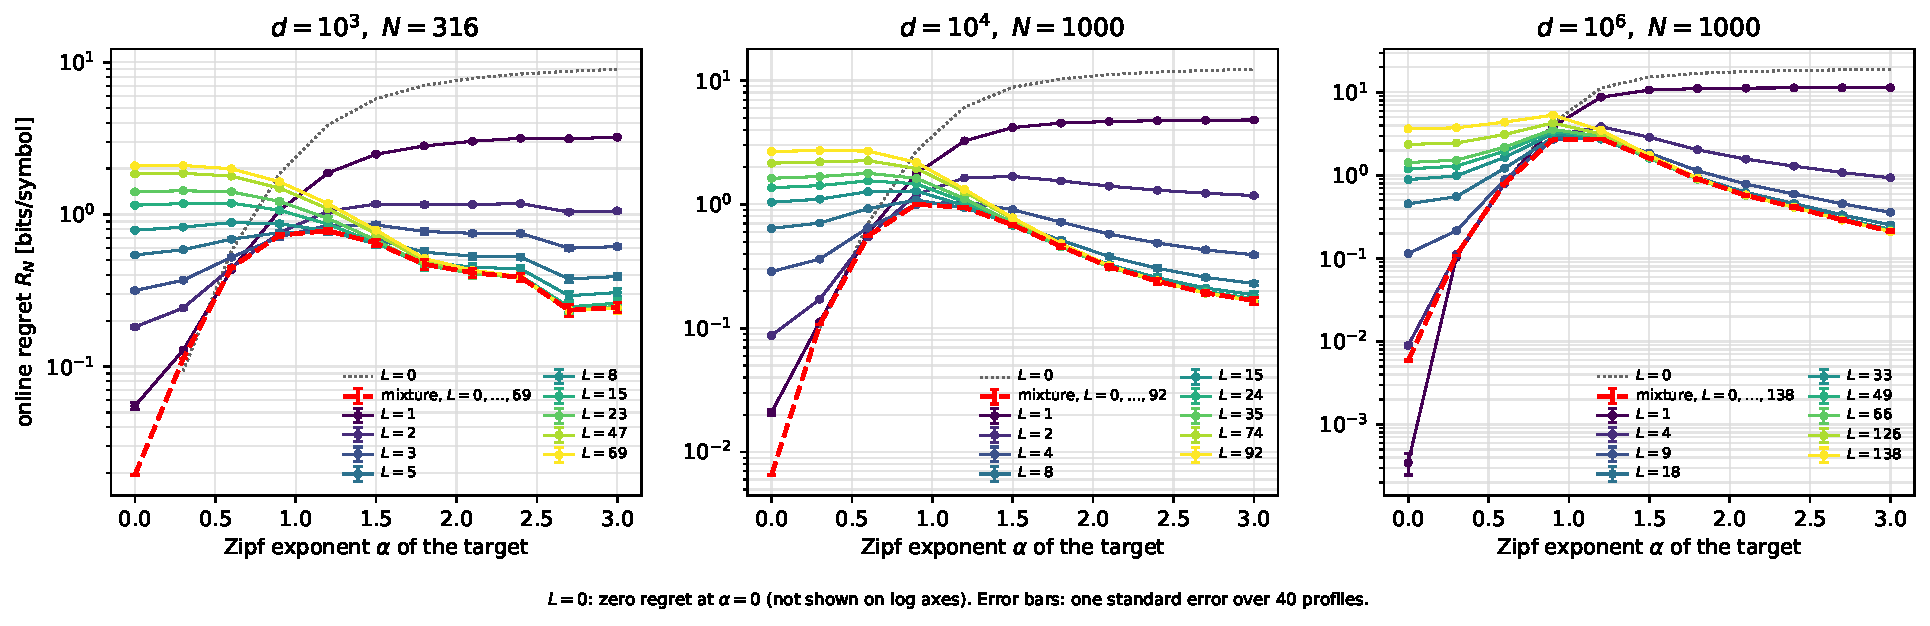
\includegraphics[width=0.95\textwidth]{figures/alt/complexity_spectrum_L0.pdf}
\caption{The best depth depends on target concentration at every alphabet size. Online regret (log scale) versus the Zipf exponent $\alpha$ of the target for $d=10^3,10^4,10^6$ ($N=316$, $1000$, $1000$). For each alphabet size, we evaluated every integer depth through $\Lmax$, where $\Lmax/\ln d\approx10$; the plot shows representative depths. Shallow depths are best for targets near uniformity. Deeper models are best as the target becomes more concentrated. Error bars: standard errors over $40$ sampled profiles.}
\label{fig:spectrum}
\end{figure*}

Figure~\ref{fig:spectrum} shows the benefit of mixing depths on Zipf targets with $d\in\{10^3,10^4,10^6\}$. For these three alphabet sizes, we use every integer depth through the corresponding $\Lmax\in\{69,92,138\}$, respectively, and sample $40$ profiles per point. Shallow priors perform best near uniformity; the best tested depth generally grows with target concentration and alphabet size. At $d=10^6$ and $\alpha=3$, the best tested depth reduces regret from $11.36$ at $L=1$ to $0.23$ bits per symbol, a factor of $49$. The depth average is at most $\log_2(\Lmax+1)/N$ bits per symbol worse than its best individual depth. Thus, more depth can help or hurt, depending on the target.

\section{Scaling laws from symbol discovery}
\label{sec:scaling}

This section has three steps. First, we count how many symbols the sample reveals. Second, we derive a lower bound that every label-invariant predictor must satisfy. Third, we show that the depth mixture matches the leading term of this bound.  \paragraph{How many symbols are discovered.} Let $S_N$ be the set of distinct symbols observed in $N$ independent samples from $p$. Define $K_N=|S_N|$, and let \[ k_N=\E K_N=\sum_{i\le d}\left[1-(1-p_i)^N\right] \] be its expectation. For a Zipf target, write $p=p_{d,\alpha}$, where $p_{d,\alpha}(i)=i^{-\alpha}/H_{d,\alpha}$ and $H_{d,\alpha}=\sum_{j=1}^d j^{-\alpha}$. For $\alpha>1$, set $a=N/H_{d,\alpha}$ and $a_N=a^{1/\alpha}$. Proposition~\ref{prop:discovery} gives \[ \left|k_N-\Gamma(1-1/\alpha)a_N\right| \le 1+\epsilon_P+\frac{ad^{1-\alpha}}{\alpha-1}, \] where $\epsilon_P\le[2e(1-\max_i p_i)]^{-1}$. As $N\to\infty$ with $d/N^{1/\alpha}\to\infty$, this implies \[ k_N\sim\Gamma(1-1/\alpha)\left(\frac{N}{\zeta(\alpha)}\right)^{1/\alpha} \] \citep{karlin1967central,gnedin2007notes}. Thus, when the sample is much smaller than the alphabet, the expected number of discovered symbols is of order $N^{1/\alpha}$.

\paragraph{What every predictor must pay.}
Suppose that the sample contains $K_N$ distinct symbols.
There are $\binom{d}{K_N}$ possible sets of observed symbols. Under a
label-invariant predictor, all sets of the same size have the same probability. Identifying
the observed set therefore costs $\log_2\binom{d}{K_N}$ bits. However, the source also makes this
set random. Given $K_N$, its uncertainty is
$H_P(S_N\mid K_N)$. The theorem below subtracts this source uncertainty from
the naming cost. For a uniform source,
every set of $k$ symbols is equally likely. The two terms then cancel, as they should:
the uniform predictor has zero regret.

\begin{theorem}[discovered-set decomposition]
\label{thm:support}
Let $P_N=p^N$, and let $Q_N$ be any label-invariant distribution on $\Xd^N$ that assigns positive probability to every sequence. Then
\begin{align}
\label{eq:support}
\KL(P_N\|Q_N)={}&\KL(P_{K_N}\|Q_{K_N})+\E\log_2\tbinom{d}{K_N}\nonumber\\
&-H_P(S_N\mid K_N)\nonumber\\
&+\E_{S_N}\KL\bigl(P_{X^N\mid S_N}\,\big\|\,Q_{X^N\mid S_N}\bigr),
\end{align}
Both divergence terms are nonnegative. Therefore, $\KL(P_N\|Q_N)\ge\E\log_2\binom{d}{K_N}-H_P(S_N\mid K_N)$.
\end{theorem}
Appendix~\ref{app:support} proves the result by applying the KL chain rule first to $S_N$ and then to $K_N$. Under a label-invariant $Q_N$, every support set of a given size has the same probability. For Zipf targets, the subtracted entropy term is only $O(k_N)$:
\begin{corollary}[Zipf lower bound]
\label{cor:zipf}
For $p=p_{d,\alpha}$, $\alpha>1$, $a_N\ge1$, and every label-invariant $Q_N$,
\begin{equation}
\label{eq:zipflb}
\KL(p^N\|Q_N)\;\ge\;\frac{k_N\ln(d/k_N)-C_\alpha a_N-2}{\ln 2},
\end{equation}
Here $C_\alpha=\ln2+\frac{1}{\alpha-1}+\frac{\alpha}{(\alpha-1)^2}$. If $a_N\to\infty$ and $a_N/d\to0$, then $\KL(p^N\|Q_N)\ge k_N\log_2(d/k_N)-O_\alpha(k_N)$.
\end{corollary}
If $d/N^{1/\alpha}\to\infty$, every label-invariant predictor therefore satisfies $R_N\gtrsim N^{1/\alpha-1}\log_2(d/N^{1/\alpha})$. The logarithmic factor is $\log(d/k_N)$; its simplification to $\log d$ holds to leading order when $\log N=o(\log d)$.

\paragraph{What the depth mixture achieves.}
For Zipf targets with $d/N^{1/\alpha}\to\infty$, Corollary~\ref{cor:zipf} gives the lower bound $(1-o(1))k_N\log_2(d/k_N)$ for every label-invariant predictor. The next theorem shows that the depth mixture matches this cost when the alphabet grows polynomially faster than the discovered set.
\begin{theorem}[first-order optimality of depth averaging]
\label{thm:optimal}
Fix $\alpha>1$. Let $N\to\infty$, and assume that $d=N^{\nu+o(1)}$ for some $\nu>1/\alpha$. Let $p=p_{d,\alpha}$. Let $Q_N$ be either the uniform depth average~\eqref{eq:avg}, with $\Lmax=\lceil\cstar\ln(2d)\rceil+1$, or the mixture with $\pi_L=1/[L(L+1)]$. Then
\begin{align}
\label{eq:optimal}
\KL(p^N\|Q_N)&=(1+o(1))\,k_N\log_2(d/k_N),\\
R_N(p)&\sim\frac{\Gamma(1-1/\alpha)}{\zeta(\alpha)^{1/\alpha}}\,N^{1/\alpha-1}\log_2\frac{d}{N^{1/\alpha}}.\nonumber
\end{align}
\end{theorem}
The expected number of discovered symbols grows as $N^{1/\alpha}$, whereas the average regret decays as $N^{-(1-1/\alpha)}\log N$. The factor $\log_2(d/k_N)$ is the leading naming cost per discovered symbol; this leading term is optimal among label-invariant predictors.
By symmetrization, this is also the minimax leading term over all label permutations of the Zipf target (Corollary~\ref{cor:permutation-minimax}).

\emph{Proof idea.} At comparator depth $\cstar\ln(d/k)+O(1)$, a prior event places the $k$ observed weights near $2dm_i/k$ and controls the total unseen weight. Exponential tilting bounds the expected excess code length above empirical entropy by $k_N\ln(d/k_N)+O(k_N\ln\ln d)$ nats. Mixing adds $O(\ln\ln d)$; entropy concavity and Corollary~\ref{cor:zipf} finish the argument (Appendix~\ref{app:optimal}). This comparator depth decreases with $k$, consistently with the observed downward shift for Zipf $\alpha=1.5$ in Section~\ref{sec:experiments}. It serves to bound cumulative regret; finite-sample evidence weights adapt to the full count profile.

Appendix~\ref{app:optimal} also allows larger depth cutoffs with negligible mixture penalty (Remark~\ref{rem:larger-cutoffs}).

Appendix~\ref{app:experiments} examines finite-sample scaling.

\section{Competitive comparison}
\label{sec:experiments}

\paragraph{Setup.}
We first compare estimators by their batch regret: the expected KL divergence from the target to the predictive distribution after $n$ observations. Table~\ref{tab:bench} uses $n=1{,}000<d=10{,}000$ and $20$ paired trials on eleven targets extending \citet{orlitsky2015competitive}: uniform; a step with half the symbols at $1/(2d)$ and half at $3/(2d)$; Zipf $\alpha\in\{1,1.5,2,3,4,5\}$; $p_i\propto0.998^i$; and draws from Dirichlet-$1$ and Dirichlet-$1/2$.
The baselines are add-one, KT, Ristad, the Good--Turing/empirical hybrid (GT), absolute discounting (AD), and a Bayesian symmetric Dirichlet mixture (Dir-$\tau$) with per-coordinate concentration $\tau/d=2^j$, $j=-24,\ldots,4$ ($29$ components; the standard hierarchical-Dirichlet construction, \citealp{mackay1995hierarchical,friedman1998efficient,minka2000estimating}). The natural oracle knows the true target but must assign equal probability to symbols with the same observed count. We compare the fixed depth $22=\operatorname{round}(\cstar\ln d)$ and the equal-prior average over $0$--$80$. We update the weights using the probability each depth assigns to the observed sequence. Additional details and results are given in Appendix~\ref{app:experiments}.

\begin{table*}[t]
\centering
\caption{Mean next-symbol KL loss in bits at $n=1{,}000$, $d=10{,}000$ ($20$ paired trials). LSA avg is the depth average~\eqref{eq:avg} over $L=0,\dots,80$ with equal prior weights, the uniform component included; $L=22=\operatorname{round}(\cstar\ln d)$ is a single depth. The natural oracle (last column) knows the target and gives a lower bound for every rule that assigns equal probability to symbols with equal observed counts. Bold marks the lowest loss in each row, excluding the oracle. Entries are sample means. Table~\ref{tab:powers-bench} repeats the benchmark on a second set of samples and summarizes sampling uncertainty. $^{*}$AD has infinite loss when $c_1=0<c_2$ and unseen symbols have positive target probability. When $c_1=c_2=0$, its discount is undefined. Numerical predictors were normalized before scoring.}

\label{tab:bench}
\footnotesize\setlength{\tabcolsep}{3.2pt}
\begin{tabular}{lrrrr|rr|rr|r}
\toprule
& \multicolumn{4}{c|}{classical} & \multicolumn{2}{c|}{adaptive controls} & \multicolumn{2}{c|}{LSA} & \\
target & add-1 & KT & Ristad & GT & Dir-$\tau$ & AD & $L=22$ & avg $0$--$80$ & oracle\\
\midrule
uniform & 0.0396 & 0.1089 & 0.0018 & 0.0628 & 0.0013 & 0.0590 & 1.4395 & $\mathbf{10^{-7}}$ & 0.0000\\
step & 0.2052 & 0.2615 & 0.1867 & 0.2255 & \textbf{0.1855} & 0.2500 & 1.5307 & 0.1907 & 0.1847\\
Zipf $\alpha=1$ & 1.7316 & 1.3474 & 1.0054 & 0.6542 & 0.8449 & \textbf{0.6429} & 0.9458 & 0.6638 & 0.6234\\
Zipf $\alpha=1.5$ & 3.0538 & 2.3026 & 0.5712 & 0.3685 & 0.4228 & 0.3598 & 0.3673 & \textbf{0.3580} & 0.3423\\
Zipf $\alpha=2$ & 3.3616 & 2.5252 & 0.2353 & 0.1641 & 0.1710 & 0.1619 & \textbf{0.1571} & 0.1576 & 0.1482\\
Zipf $\alpha=3$ & 3.4392 & 2.5752 & 0.0682 & 0.0510 & 0.0507 & $\infty^{*}$ & 0.0511 & \textbf{0.0484} & 0.0426\\
Zipf $\alpha=4$ & 3.4509 & 2.5814 & 0.0305 & 0.0233 & 0.0224 & n.a.$^{*}$ & 0.0240 & \textbf{0.0217} & 0.0185\\
Zipf $\alpha=5$ & 3.4542 & 2.5828 & 0.0146 & 0.0128 & \textbf{0.0110} & n.a.$^{*}$ & 0.0140 & 0.0114 & 0.0087\\
geometric & 2.2297 & 1.9719 & \textbf{1.5664} & 1.6021 & 1.5969 & 1.6759 & 1.8023 & 1.6373 & 1.5625\\
Dirichlet-$1$ & \textbf{0.5625} & 0.5829 & 0.5635 & 0.5892 & 0.5629 & 0.6370 & 1.6854 & \textbf{0.5625} & 0.5623\\
Dirichlet-$\frac12$ & 0.9107 & \textbf{0.8887} & 0.8902 & 0.9240 & \textbf{0.8887} & 0.9683 & 1.7953 & 0.8998 & 0.8882\\
\bottomrule
\end{tabular}
\end{table*}

\begin{table*}[t]
\centering
\caption{Compressing the King James Bible ($d=10^5$).
Redundancy in bits per token above the empirical
unigram entropy $\hat H_n$ for prefixes of $n$ tokens.
LSA avg uses equal prior weights over $L=0,\ldots,54$.
Bold marks the lowest redundancy at each prefix.}
\label{tab:bible}
\small\setlength{\tabcolsep}{5pt}
\begin{tabular}{rrcccccccc}
\toprule
$n$ & distinct & $\hat H_n$
& add-1 & KT & Ristad & GT
& Dir-$\tau$ & LSA avg & post.\ mode\\
\midrule
$10{,}000$ & 1{,}160 & 7.56
& 4.597 & 3.846 & 1.193 & 1.066
& 1.081 & \textbf{1.052} & $L=21$\\
$30{,}000$ & 2{,}119 & 7.87
& 3.225 & 2.512 & 0.709 & 0.606
& 0.621 & \textbf{0.598} & $L=21$\\
$100{,}000$ & 3{,}839 & 8.02
& 1.911 & 1.359 & 0.381 & 0.310
& 0.317 & \textbf{0.306} & $L=21$\\
$300{,}000$ & 6{,}922 & 8.18
& 1.026 & 0.679 & 0.224 & 0.170
& 0.176 & \textbf{0.168} & $L=19$\\
$915{,}860$ & 13{,}550 & 8.48
& 0.478 & 0.303 & 0.137 & 0.097
& 0.102 & \textbf{0.095} & $L=15$\\
\bottomrule
\end{tabular}
\end{table*}

\begin{figure*}[t]
\centering
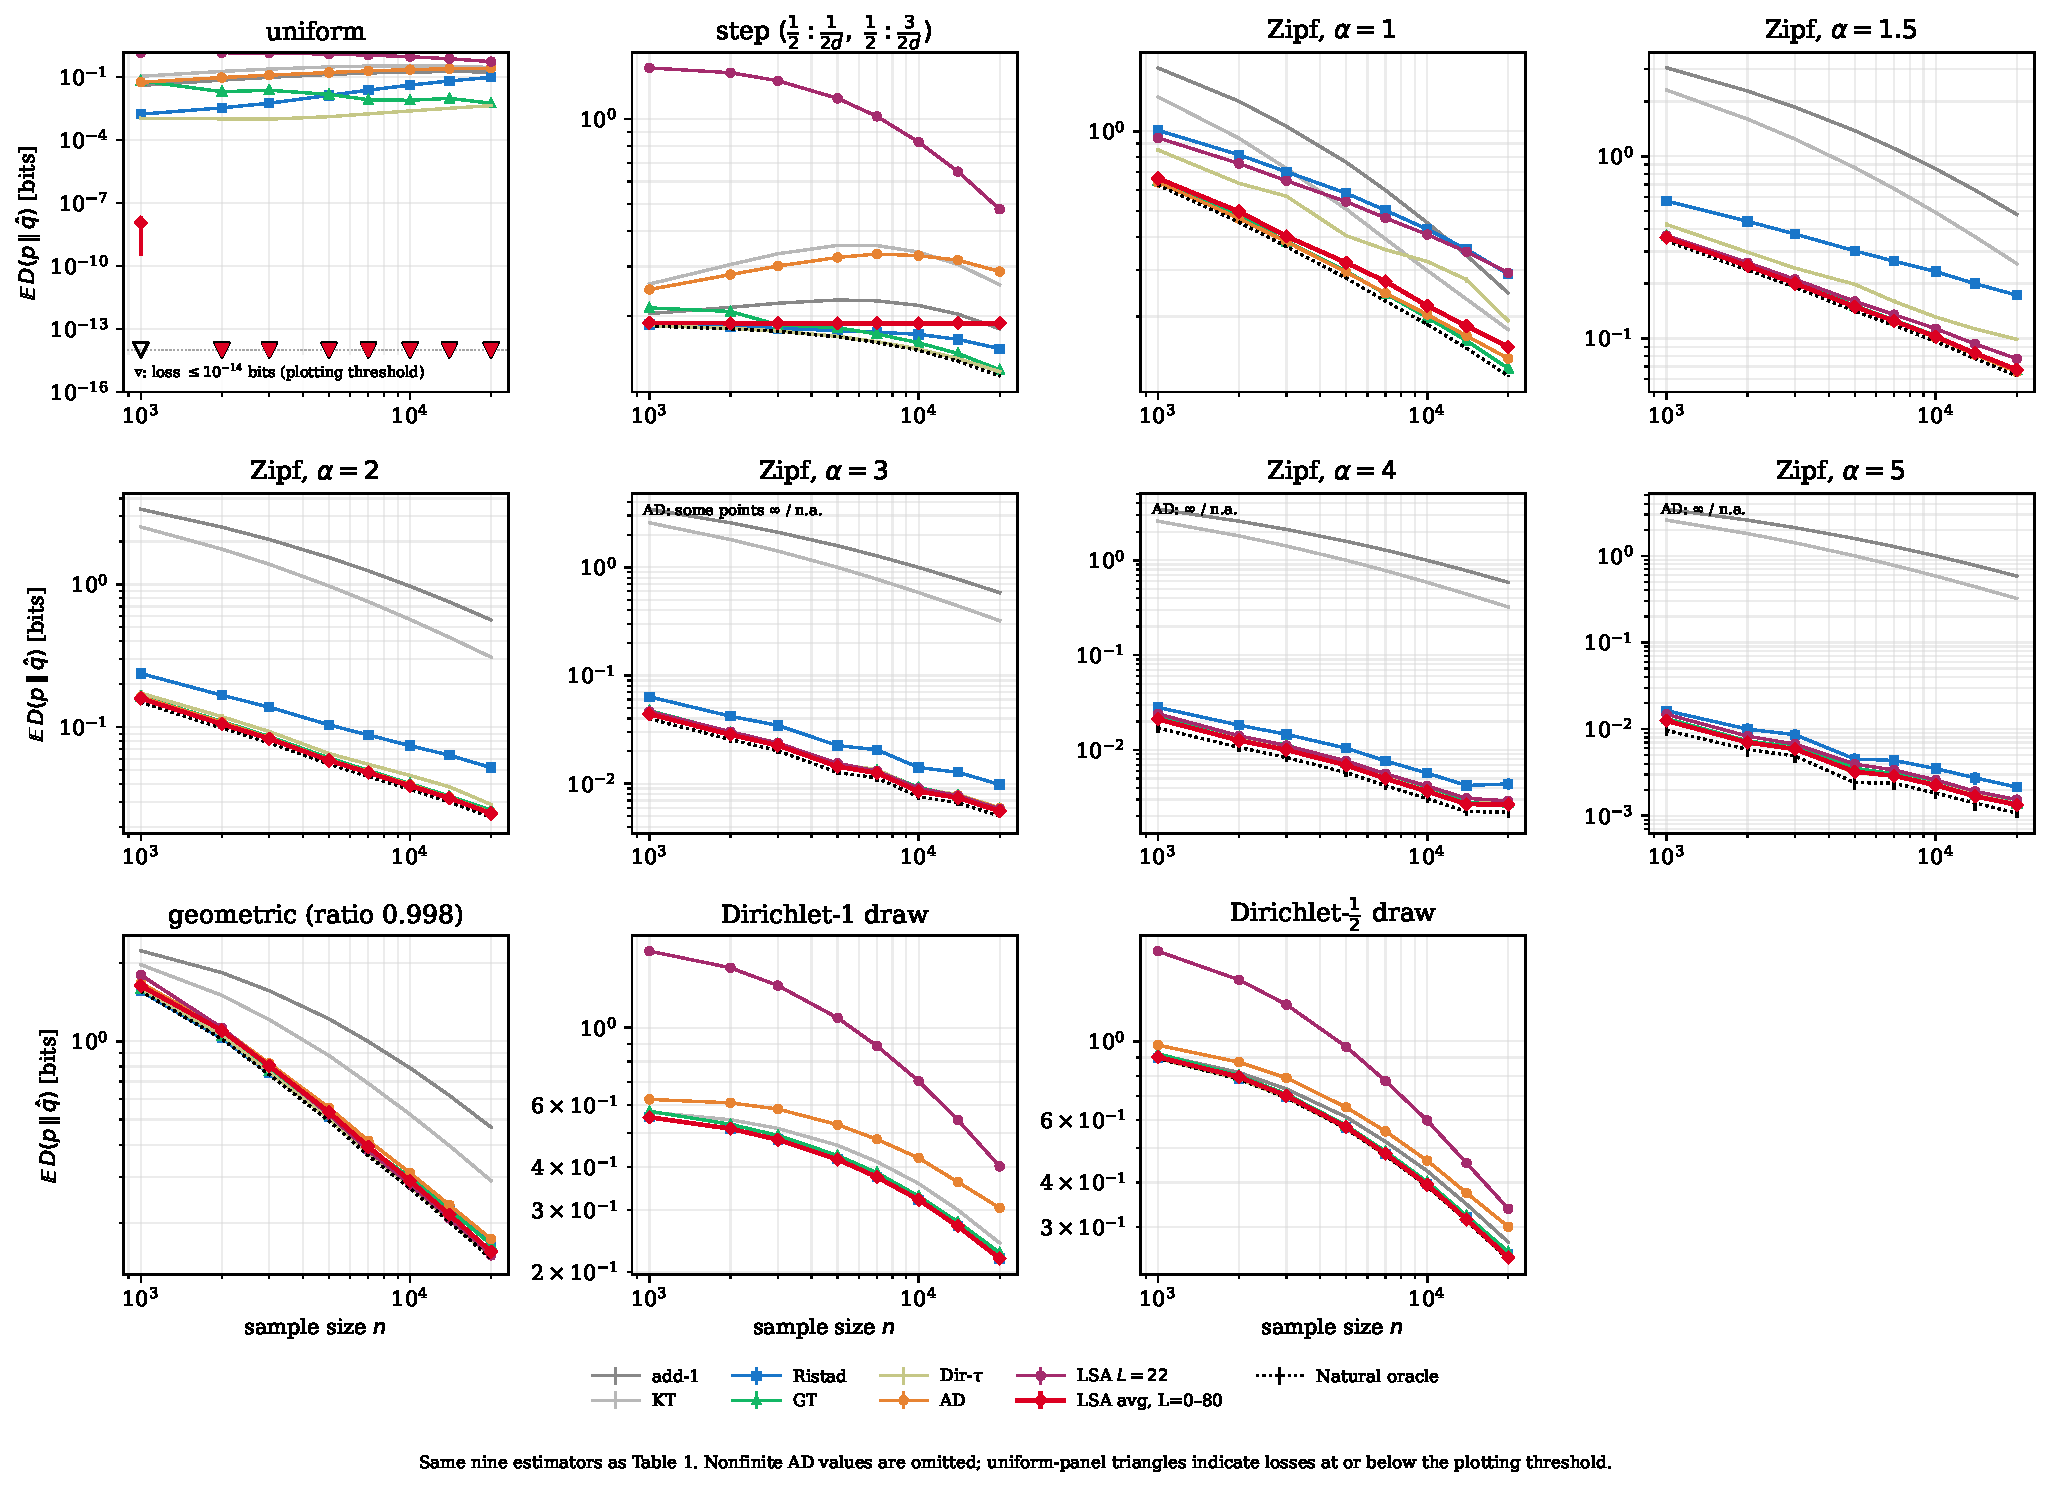
\includegraphics[width=\linewidth]{figures/alt/regret_vs_n_figures.pdf}
\caption{Competitive comparison on the benchmark of \citet{orlitsky2015competitive} extended to eleven targets ($d=10^4$; log-log axes; $20$ trials, standard-error bars). The mixture LSA predictor (red diamonds) is competitive on practically all targets. On the uniform target its loss is much lower, due to the $L=0$ component. In the uniform panel, downward triangles mark losses at or below $10^{-14}$ bits. }
\label{fig:orlitsky}
\end{figure*}

\paragraph{Findings.}
At $n=1{,}000$ and $d=10{,}000$, the average over depths $0$--$80$ has the lowest loss among the non-oracle rules, or ties it at the displayed precision, on five of the eleven targets (Table~\ref{tab:bench}). Its mean is within $5\%$ of the lowest on all other targets. Figure~\ref{fig:orlitsky} compares the methods at the tested sample sizes from $10^3$ to $2\cdot10^4$. On the Zipf targets with $\alpha\ge1.5$, the LSA mean is below Good--Turing's in both runs: by $3$--$11\%$ in Table~\ref{tab:bench} and $1.5$--$7\%$ in Table~\ref{tab:powers-bench}. At $\alpha=1$, Good--Turing's mean is lower by about $1.5\%$ and $2.4\%$, respectively. For $\alpha\ge3$, the gaps among the strongest methods are comparable in scale to the differences between the two runs. The gain over add-constant rules is large: at $\alpha=2$, add-one and KT incur $3.3616$ and $2.5252$ bits against $0.1576$. Including the uniform component mainly improves the uniform and step targets in these experiments. Compared with the positive-depth average, the loss falls from $0.0396$ to below $0.001$ bits on the uniform target and from $0.2052$ to $0.1907$ bits on the step target. The cumulative mixture penalty increases from $\log_2 80$ to $\log_2 81$ bits.

\emph{Comparison with the Dirichlet mixture.} The Dir-$\tau$ control adapts the concentration of a symmetric Dirichlet prior by the same evidence rule as depth, providing an adaptive-prior comparison. LSA includes an exact uniform component; the Dirichlet control approaches uniformity through its largest finite concentrations. In Table~\ref{tab:bench}, on identical samples, the LSA mean is below the Dirichlet mean on Zipf $\alpha=1$ to $4$ (by $21$, $15$, $8$, $4.5$ and $3\%$), is nearly equal to it on Dirichlet-1, and is $1$--$4\%$ above it only on the step, geometric, Dirichlet-$\tfrac12$ and Zipf-$5$ targets. The largest gains over the Dirichlet mixture occur on the tested Zipf targets with the smallest $\alpha$. 

Good--Turing and the LSA mixture both use the count profile, but estimate the probability mass of each count class differently. Good--Turing uses the numbers of symbols with neighboring counts. The Bayesian mixture combines the observed counts with its prior (Appendix~\ref{app:regret}). Table~\ref{tab:posteriors} (Appendix~\ref{app:experiments}) shows how the depth weights adapt. They favor $L=0$ on the uniform and step targets. For Zipf $\alpha=1.5$, most weight lies on depths $12$--$19$ at $n=1{,}000$, and on depths $9$--$10$ at $n=20{,}000$. This decrease is consistent with the depth scale $\cstar\ln(d/k)$ used in the proof of Theorem~\ref{thm:optimal}. For $\alpha\ge3$, the weights remain spread over many large depths. 

\paragraph{Real text: compressing the King James Bible.}
The text experiment uses the King James Bible (Project Gutenberg \#10), with $915{,}860$ word-and-punctuation tokens and $13{,}550$ distinct types, embedded in an alphabet of $d=10^5$. The alphabet accommodates the corpus vocabulary and a reservoir of unseen labels. The metric is cumulative coding redundancy: code length per token minus the empirical unigram entropy of the prefix. On the full corpus, LSA uses $0.095$ extra bits per token, Good--Turing $0.097$, and the Dirichlet mixture $0.102$, a span of $0.007$ bits per token (Table~\ref{tab:bible}). Good--Turing has a lower redundancy on the short prefixes in Appendix~\ref{app:experiments}. The LSA posterior mode decreases from $21$ to $15$. The code lengths condition on a token dictionary and tokenization rule.

\section{Related work and discussion}
\label{sec:discussion}

\paragraph{Large-alphabet estimation.} Good--Turing~\citep{good1953population,gale1995good} and its analyses~\citep{orlitsky2003always,mcallester2000leave,acharya2013tight,orlitsky2015competitive,valiant2016instance,ohannessian2012rare,falahatgar2017power}, Pitman--Yor models~\citep{teh2006hierarchical}, and hierarchical Dirichlet priors with a learned or mixed concentration parameter~\citep{mackay1995hierarchical,friedman1998efficient,hutter2013sparse} address the same problem. Methods for assigning probability to unseen symbols, including prediction by partial matching (PPM) and absolute discounting~\citep{cleary1984data,witten1991zero}, are also relevant. Our evidence formula~\eqref{eq:gammatrick} is related to posterior analysis of normalized random measures~\citep{james2009posterior}. The LSA predictor satisfies bound~\eqref{eq:priormass}. For the Zipf targets covered by Theorem~\ref{thm:optimal}, the depth mixture achieves the best leading-order regret among label-invariant codes. The experiments in Section~\ref{sec:experiments} assess competitiveness across a broader range of targets. For a fixed alphabet, KT~\citep{krichevsky1981performance} achieves the optimal leading term in worst-case cumulative regret as the sample size grows~\citep{xie2000asymptotic}. However, it can be costly when only a small fraction of the alphabet is observed.

\paragraph{Discovery and coding redundancy.}
The pattern--dictionary decomposition separates repetition structure from symbol identities~\citep{orlitsky2004unknown}. \citet{falahatgar2015universal} establish order bounds for unordered power-law classes when $d>N$. Applying the Zipf count estimates in Appendix~\ref{app:optimal} to the adaptive sparse-predictor bound of \citet[Theorem~5]{hutter2013sparse} also yields the leading upper bound $k_N\log_2(d/k_N)$. That adaptive process generally depends on observation order. Our result establishes the sharp constant for an exchangeable predictor from a fixed Bayesian depth mixture, for fixed $\alpha>1$ and $d=N^{\nu+o(1)}$, $\nu>1/\alpha$; this regime includes $d<N$. Both LSA and existing adaptive sparse predictors operate without knowing $\alpha$.

\paragraph{Scope.}
Theorem~\ref{thm:optimal} characterizes the leading term of expected cumulative regret for fixed $\alpha>1$ as $d=N^{\nu+o(1)}$ grows with $N$, where $\nu>1/\alpha$. Finite-sample behavior is examined through the empirical approximation~\eqref{eq:law} and the single-weight heuristic in Appendix~\ref{app:experiments}. The text evaluation uses the King James Bible as a case study. Powered layers preserve the evidence representation; the optimality result concerns unit-power depth mixtures.

\section{Conclusion}
LSA combines a simple multiplicative construction, explicit evidence and regret expressions, and competitive prediction across the tested sources. The evidence representation supports numerical evaluation and analysis of how depth shapes the prior. For the Zipf regime studied here, the depth mixture also attains the sharp leading-order discovery cost. Powered layers preserve the evidence representation.

\clearpage

\section*{AI Disclosure}
Generative AI tools were used to assist implementation of the numerical methods and experiment drivers (Claude, Anthropic), formulation and refinement of claims and proofs (Claude and ChatGPT, OpenAI), experimental design and critique, independent numerical checks, and interpretation of results. They were also used to draft and edit the manuscript, identify literature, format references, and prepare figures. ChatGPT also assisted consistency and layout checks. The authors reviewed the AI-assisted proofs by hand and are responsible for the manuscript's claims, results, and AI-assisted content.

\bibliography{references_shorter}

\clearpage
\appendix

\section{Prior-mass and regret identities}
\label{app:regret}

\begin{proofof}{the prior-mass bound~\eqref{eq:priormass}}
Fix $N\ge1$ and $\epsilon\ge0$ with $w_\epsilon=w(\Theta_0^\epsilon)>0$. Let $w_B$ be the prior restricted to $\Theta_0^\epsilon$ and normalized to have total mass one. For every $x^N$ with $p^N_{\theta_0}(x^N)>0$, $Q_N(x^N)\ge w_\epsilon\,p^N_{\theta_0}(x^N)\,\E_{\theta\sim w_B}[p^N_\theta(x^N)/p^N_{\theta_0}(x^N)]$. Apply $-\log_2$ to both sides. Since this function is convex, Jensen's inequality and expectation under $p^N_{\theta_0}$ give \[\KL(p^N_{\theta_0}\|Q_N)\le-\log_2w_\epsilon+N\,\E_{w_B}\KL(p_{\theta_0}\|p_\theta)\le-\log_2w_\epsilon+N\epsilon.\] Divide by $N$ and take the infimum over $\epsilon$ (zero mass gives an infinite bound).
\end{proofof}

\begin{proofof}{Theorem~\ref{thm:regret}}
For $X^N\sim p^N$ iid, $\E\log_2 p^N(X^N)=\sum_t\E\log_2p(X_t)=-NH(p)$. Hence
$\frac1N\KL(p^N\|Q_N)=\frac1N\E\log_2p^N(X^N)-\frac1N\E\log_2Q_N(X^N)=-H(p)-\frac1N\E\log_2 q_{M}$ with $M=m(X^N)\sim\Mult(N,p)$. Since $q_m$ depends on $m$ only through $\profile(m)$, grouping count vectors by profile gives~\eqref{eq:regret}. For the batch regret, $\hat q_m(i)=Q(X_{N+1}=i\mid X^N)=Q_{N+1}(x^N i)/Q_N(x^N)=q_{m+e_i}/q_m$, and $\KL(p\|\hat q_m)=-H(p)-\sum_ip_i\log_2\hat q_m(i)$. For fixed $m$, symbols with the same observed count have equal predictive probabilities. These probabilities may depend on the entire profile. Grouping over $r\ge0$ with $c_r>0$ gives~\eqref{eq:batch}; the unseen class is included when present. For $N=0$, $q_0=1$ and symmetry gives $\hat q_0(i)=1/d$. The identity \[\sum_iq_{m+e_i}=\E\Bigl[\prod_j\theta_j^{m_j}\sum_i\theta_i\Bigr]=q_m\] shows that the predictive probabilities sum to one. It also shows that summing over the last symbol in $Q_{N+1}$ gives $Q_N$. The chain rule $Q_N(x^N)=\prod_{n<N}\hat q_{m(x^n)}(x_{n+1})$ under the iid target then gives $\KL(p^N\|Q_N)=\sum_{n<N}\E\KL(p\|\hat q_{M_n})$, i.e.\ $NR_N=\sum_{n<N}\batchreg_n$.
\end{proofof}

\paragraph{The natural oracle.}
Fix a count vector $m$. For each nonempty count class $C_r=\{i:m_i=r\}$, let $c_r=|C_r|$ and $S_r=\sum_{i\in C_r}p_i$, including $r=0$ when symbols are unobserved. A natural estimator assigns $\hat q_m(i)=z_r$ within this class, with total estimated probability $T_r=c_rz_r$. The natural oracle assigns $q^*_m(i)=S_r/c_r$. Adding and subtracting $\log_2(S_r/c_r)$ within each class with $S_r>0$ gives
\begin{equation}
\KL(p\|\hat q_m)=\KL(p\|q^*_m)+\KL\bigl((S_r)_r\big\|(T_r)_r\bigr).
\end{equation}
Classes with $S_r=0$ contribute zero. If $T_r=0<S_r$, both sides are infinite. The second term is nonnegative, so the oracle minimizes KL loss among natural estimators. This term also gives the excess loss of any natural estimator over the oracle.

\begin{proofof}{Proposition~\ref{prop:laplace}}
For $\theta\sim\Dir(a_1,\dots,a_d)$, $\E\prod_i\theta_i^{m_i}=\frac{\Gamma(\sum_ia_i)}{\Gamma(\sum_i a_i+N)}\prod_i\frac{\Gamma(a_i+m_i)}{\Gamma(a_i)}$. With $a_i\equiv1$ this is $\Gamma(d)\prod_im_i!/\Gamma(d+N)$, and \[\frac{q_{m+e_i}}{q_m}=\frac{(m_i+1)!}{m_i!}\cdot\frac{\Gamma(d+N)}{\Gamma(d+N+1)}=\frac{m_i+1}{N+d}.\]
\end{proofof}

\begin{proofof}{Proposition~\ref{prop:avg}}
$Q_N(x^N)\ge\pi_LQ^{(L)}_N(x^N)$ pointwise; take $-\log_2$, then the expectation under $p^N$, and divide by $N$. The same argument holds for a mixture over infinitely many depths. Nonnegative weights that sum to one give a valid probability distribution. For the proposed weights, \[\sum_{L=1}^{\infty}\frac{1}{L(L+1)}=\sum_{L=1}^{\infty}\left(\frac1L-\frac1{L+1}\right)=1.\]
\end{proofof}
For a given sequence, the code-length bound for depth $L$ is nearly attained when that depth's posterior weight is close to one. Positive prior weights and likelihoods give positive posterior weights at every finite sample size. The bound controls cumulative regret. The next-symbol regret is the increment $\batchreg_N=(N+1)R_{N+1}-NR_N$, which we evaluate separately.

\section{Computing the mixture weights \texorpdfstring{$q_\lambda$}{q-of-lambda}
 and the predictive probabilities}
\label{app:qlambda}

\paragraph{Integral representation.} The quantity to compute is $q_\lambda=\E\prod_i\theta_i^{m_i}$ with $\theta_i=Y_i/S$ and $S=\sum_jY_j$. The $Y_i$ are independent, but the common denominator $S^{N}$ couples them. The definition of the Gamma function, $\Gamma(N)=\int_0^\infty u^{N-1}e^{-u}du$, with the substitution $u=tS$ gives
\begin{equation}
S^{-N}=\frac{1}{\Gamma(N)}\int_0^\infty t^{N-1}e^{-tS}\,dt\qquad(N\ge1,\ S>0),
\end{equation}
which replaces the denominator by an exponential of a \emph{sum}. Since $S>0$ almost surely and every factor below is nonnegative, Tonelli's theorem allows the expectation and the $t$-integral to be interchanged, and the exponential factorizes over the independent $Y_i$:
\begin{equation}
\label{eq:q-integral}
q_\lambda=\E\Bigl[S^{-N}\prod_iY_i^{m_i}\Bigr]=\frac1{\Gamma(N)}\int_0^\infty t^{N-1}\prod_i\E\bigl[Y_i^{m_i}e^{-tY_i}\bigr]dt=\frac1{\Gamma(N)}\int_0^\infty t^{N-1}\prod_{r\ge0}\phi_r(t)^{c_r}\,dt,
\end{equation}
with $\phi_r(t)=\E[Y^re^{-tY}]$, where $Y=\prod_{\ell=1}^LE_\ell$ is the unnormalized weight for one symbol; the last step groups the $c_r$ symbols with count $r$ (including the $c_0$ unseen ones, each contributing $\phi_0$). The factorization uses the independence of the unnormalized $Y_i$; the common normalizer couples the $\theta_i$. For $N=0$, set $q_0=1$ directly. The same reduction applies to independent nonnegative weights whose sum is positive almost surely. If the weights have the same distribution, their factors can again be grouped by count. This Laplace-transform method also appears in normalized random measures~\citep{james2009posterior}. The layered architecture enters only through the distribution of $Y$ and the functions $\phi_r$.

\paragraph{Kernel rows by a layer recursion.} Write $Y=E\cdot V$, where $E\sim\Exp(1)$ is the last layer and $V$ is the product of the other $L-1$. Conditioning on $E=x$ turns $\E[Y^re^{-tY}]$ into $x^r\,\E[V^re^{-(tx)V}]=x^r\phi^{(L-1)}_r(tx)$, so averaging over $x$ gives
\begin{equation}
\label{eq:phi-recursion}
\phi^{(\ell)}_r(t)=\int_0^\infty e^{-x}x^r\,\phi^{(\ell-1)}_r(tx)\,dx,\qquad \phi^{(1)}_r(t)=\int_0^\infty y^re^{-(1+t)y}\,dy=\frac{\Gamma(r+1)}{(1+t)^{r+1}} .
\end{equation}
Adding a layer is thus one integral applied to the previous row, independent of $d$ and of the profile, and evaluating depth $L$ produces every shallower depth on the way. A single recursion chain shares kernel work across depths; evidence integration, aggregation, profile processing and accuracy requirements still incur costs that depend on $d$ and the sample. As a check, at $L=1$ the rows are explicit and~\eqref{eq:q-integral} becomes $\frac{\prod_i\Gamma(m_i+1)}{\Gamma(N)}\int_0^\infty t^{N-1}(1+t)^{-(N+d)}dt=\prod_im_i!\,B(N,d)/\Gamma(N)=\prod_im_i!\,\Gamma(d)/\Gamma(d+N)$, the Dirichlet$(1,\dots,1)$ moment formula of Proposition~\ref{prop:laplace}.

\paragraph{Kernel rows by a Mellin--Barnes contour.} Numerical errors can accumulate across layers. In the logarithm of the integrand in~\eqref{eq:q-integral}, the error in $\ln\phi_0$ is multiplied by $c_0$. For small $r$, we therefore evaluate $\phi_r$ directly using the contour formula below. It rests on two facts. First, the Mellin transform of $Y$ factorizes: $\E[Y^{z-1}]=\prod_{\ell}\E[E_\ell^{z-1}]=\Gamma(z)^L$ for $\Re z>0$. Second, the exponential has the inverse-Mellin (Cahen--Mellin) representation
\begin{equation}
e^{-u}=\frac{1}{2\pi i}\int_{\sigma-i\infty}^{\sigma+i\infty}\Gamma(z)\,u^{-z}\,dz,\qquad \sigma>0,
\end{equation}
which is Mellin inversion of $\int_0^\infty u^{z-1}e^{-u}du=\Gamma(z)$. Inserting it with $u=tY$ into $\phi_r(t)=\E[Y^re^{-tY}]$ and taking the expectation inside,
\begin{equation}
\label{eq:mb}
\phi_r^{(L)}(t)=\frac1{2\pi i}\int_{\sigma-i\infty}^{\sigma+i\infty}\Gamma(z)\,t^{-z}\,\E\bigl[Y^{r-z}\bigr]\,dz=\frac1{2\pi i}\int_{\sigma-i\infty}^{\sigma+i\infty}\Gamma(z)\,\Gamma(r+1-z)^L\,t^{-z}\,dz,
\end{equation}
since $\E[Y^{r-z}]=\Gamma(1+r-z)^L$ exists for $\Re(r-z)>-1$. For $0<\sigma<r+1$, \[t^{-\sigma}\E[Y^{r-\sigma}]\int_{\mathbb R}|\Gamma(\sigma+iy)|\,dy<\infty.\] This bound justifies exchanging expectation and integration. The valid strip $0<\sigma<r+1$ has its left edge from the Cahen--Mellin integral and its right edge from the existence of the moment. On a vertical line $|t^{-z}|=t^{-\sigma}$ is constant and, by Stirling's formula, $|\Gamma(\sigma+iy)|\sim\sqrt{2\pi}\,|y|^{\sigma-1/2}e^{-\pi|y|/2}$, so the integrand decays like $e^{-(L+1)\pi|y|/2}$ times a polynomial. The exponential decay becomes faster as $L$ increases. Moving the contour across a pole requires the residue: crossing $z=0$ to the left contributes $\Gamma(r+1)^L$, which the implementation extracts explicitly to avoid cancellation at small $t$ (where $\phi_r\to\Gamma(r+1)^L$); crossing the order-$L$ pole at $z=r+1$ to the right gives the fixed-parameter tail $\phi^{(L)}_r(t)=\frac{\Gamma(r+1)}{(L-1)!}\,t^{-(r+1)}(\ln t)^{L-1}[1+o(1)]$ as $t\to\infty$, whose leading constant depends on $r$ and $L$. Let $a\approx1.4616$ minimize $\log\Gamma(a)$ for $a>0$. The contour is placed at $\sigma=r+1-a$. For $r\ge1$, this lies in the original strip. For $r=0$, it lies to the left of $z=0$, so the residue term $\Gamma(r+1)^L$ must be added. The rows show step-halving agreement below $3\cdot10^{-9}$ for all small $r$ at every depth used ($L\le138$), match independent Meijer-G evaluations where those converge, and provide direct kernel evaluations for small $r$.

\paragraph{Numerical scheme.}
All computations store $h_r(u)=\ln\phi_r(e^u)$ on a uniform grid in $u=\ln t$. With $v=\ln x$, the integration weight is $\exp((r+1)v-e^v)$. Its peak has approximate width $(r+1)^{-1/2}$ in $v$. For large $t$, the full integrand also has a broad, slowly varying region. The scheme integrates these two regions separately and combines the results. The outer integral is evaluated in the log domain: with $\Psi_m(u)=Nu+(d-s)h_0(u)+\sum_{r\ge1}c_rh_r(u)$ (the term $Nu$ absorbs $t^{N-1}$ and the Jacobian), $q_m=\frac1{\Gamma(N)}\int e^{\Psi_m(u)}du$ and, using $\Gamma(N+1)=N\Gamma(N)$,
\begin{equation}
\hat q_m(i)=\frac{q_{m+e_i}}{q_m}=\frac1N\cdot\frac{\int e^{u}\,\bigl(\phi_{r+1}/\phi_r\bigr)(e^u)\,e^{\Psi_m(u)}\,du}{\int e^{\Psi_m(u)}\,du}\qquad(r=m_i,\ N\ge1),
\end{equation}
Thus, the numerator uses the same integrand, with one factor $\phi_r$ replaced by $\phi_{r+1}$ and an extra factor $t$. For $N=0$, symmetry gives $\hat q_0(i)=1/d$. Counts up to $m_{\max}\approx2\cdot10^4$ arise on the benchmark (the top symbol of Zipf $\alpha=5$ at $n=2\cdot10^4$); tables store directly computed values for all small counts and anchor rows at geometric spacing above, and a missing row is interpolated through bracketing anchors after removing a known smooth trend, with errors $\sim10^{-4}$ in $h_r$ and $\sim2\cdot10^{-5}$ in predictive differences.

\paragraph{Error propagation.}
If approximate log-kernels satisfy $|\tilde h_r-h_r|\le\epsilon_r$ on the whole integration domain (including a rigorously bounded tail), then with $\Delta_m=(d-s)\epsilon_0+\sum_{r\ge1}c_r\epsilon_r$, pointwise exponentiation gives $e^{-\Delta_m}Z_m\le\tilde Z_m\le e^{\Delta_m}Z_m$ for $Z_m=\int e^{\Psi_m}$; if the quadrature has relative error at most $\eta<1$, then $|\ln\tilde q_m-\ln q_m|\le\Delta_m-\ln(1-\eta)$. The log error in a predictive ratio is at most the sum of the log errors in its numerator and denominator. If every depth has log-evidence error at most $\delta$, then the mixture's log-evidence error is at most $\delta$. Each posterior log-weight has error at most $2\delta$. The zero-count kernel error is amplified by $d-s$, which is why the rows computed from~\eqref{eq:mb} are used for small $r$ at large $d$; Appendix~\ref{app:validation} gives complementary numerical checks. 

\section{Computing the profile weights \texorpdfstring{$A_{\lambda}(p)$}{A-of-lambda(p)}}
\label{app:alambda}
Let $\lambda$ have positive-count multiplicities $c_r$, $r\ge1$, with $\sum_{r\ge1}rc_r=N$, $\mathcal R_\lambda=\{r\ge1:c_r>0\}$ and $s=\sum_{r\ge1}c_r$ ($A_\lambda=0$ if $s>d$). Each symbol is either unused, contributing $1$, or used $r$ times, contributing $z_rp_i^r/r!$, so
\[
A_\lambda(p)=\Gamma(N+1)\,[z^c]\prod_{i=1}^d\Bigl(1+\sum_{r\in\mathcal R_\lambda}z_r\frac{p_i^r}{\Gamma(r+1)}\Bigr),
\]
where $[z^c]$ denotes the coefficient of $\prod_{r\in\mathcal R_\lambda}z_r^{c_r}$. The unused class has size $c_0=d-s$ and is represented by the constant term. For the uniform target $u_i=1/d$, the formula becomes \[A_\lambda(u)=\frac{\Gamma(N+1)}{d^N}\frac{d!}{(d-s)!}\prod_{r\ge1}\frac{1}{\Gamma(r+1)^{c_r}c_r!}.\] By symmetry, the coefficient is a polynomial in the sums $P_j=\sum_i p_i^j$, with $1\le j\le N$. We evaluate this polynomial recursively after computing the required sums. The computational cost can depend on $d$. For large $N$, we evaluate the expectation in~\eqref{eq:regret} by drawing $M\sim\Mult(N,p)$ and average the computed $\log_2 q_M$ values. The Monte Carlo average is unbiased for exact log-probabilities; Appendix~\ref{app:qlambda} separately quantifies numerical error propagation. The identity $\sum_\lambda A_\lambda=1$ and the formula for a uniform target provide checks on the computation. The description length $\E\log_2\binom{d}{K_N}$ in Section~\ref{sec:scaling} is estimated from the same sampled profiles. For comparison, we also compute the corresponding expectation when the sample size has a Poisson distribution with mean $N$. In that model, the distribution of the number of distinct symbols is computed recursively over the alphabet.

\section{The role of the depth}
\label{app:fixedd}

This appendix shows how depth changes the prior over probability vectors with $d$ coordinates. We first study $L$ proportional to $\ln d$. We then study the limits with either $L$ or $d$ fixed. 

\paragraph{Large-deviation calculation.} For logarithmic depth \(L=\lfloor c\ln d\rfloor\), with \(c>0\), consider a single unnormalized weight \(Y=\prod_{\ell=1}^{L}E_\ell\), where the \(E_\ell\) are independent unit exponentials. Define
\[
I(x)=\sup_{\beta>-1}\{\beta x-\ln\Gamma(1+\beta)\},
\qquad
\rho_0(c)=cI(1/c).
\]
Since \(\ln Y\) is a sum of independent log-exponential variables, Cramér’s theorem gives
\[
\Pr\{Y\ge d\}=d^{-\rho_0(c)+o(1)}
\qquad(d\to\infty).
\]
Thus, \(\rho_0(c)\) quantifies the probability cost of a prescribed unnormalized weight reaching the scale \(d\).

\paragraph{Properties of $\rho_0(c)$.} Let $\Lambda(\beta)=\ln\Gamma(1+\beta)$. Write $\psi(x)=\frac{d}{dx}\ln\Gamma(x)$ and $\psi_1(x)=\psi'(x)$. Then $\Lambda'(\beta)=\psi(1+\beta)$ and $\Lambda''(\beta)=\psi_1(1+\beta)>0$, so $\Lambda$ is strictly convex for $\beta>-1$. For $x>-\gamma$ the maximizer $\beta(x)$ in $\rate(x)=\sup_\beta[\beta x-\Lambda(\beta)]$ solves $\psi(1+\beta)=x$, and $\rate'(x)=\beta(x)$, $\rate''(x)=1/\psi_1(1+\beta(x))$. With $x=1/c$, $\rho_0'(c)=\rate(x)-x\rate'(x)=-\Lambda(\beta(1/c))$ and $\rho_0''(c)=1/[c^3\psi_1(1+\beta(1/c))]$. Since $\Lambda<0$ on $(0,1)$, $\Lambda(1)=0$ and $\Lambda>0$ beyond, and $\beta(1/c)$ decreases in $c$, $\rho_0$ decreases until $\beta(1/c)=1$, i.e.\ $1/c=\psi(2)=1-\gamma$, and increases afterwards; at $\cstar=1/(1-\gamma)$ its value is $\cstar[(1-\gamma)-\Lambda(1)]=1$ and $\rho_0''(\cstar)=(1-\gamma)^3/\psi_1(2)=(1-\gamma)^3/(\pi^2/6-1)\approx0.1172$. Numerically $\rho_0(1)=1.315$, $\rho_0(1.5)=1.075$, $\rho_0(2)=1.009$. As $x\to\infty$, Stirling's formula gives $\rate(x)\sim e^x$. Hence $\rho_0(c)\sim c e^{1/c}$ as $c\to0$. The rate function $\rate$ is applied to the average log weight $(\ln Y)/L$. Its threshold $(\ln d)/L$ tends to $1/c$. The mean of this average is $-\gamma$. Related joint asymptotics for normalized weights are studied by \citet{jeong2026phase}. Appendix~\ref{app:optimal} gives the self-contained regret argument; Appendix~\ref{app:experiments} explores a heuristic connection between $\rho_0$ and finite-sample regret.

\paragraph{Fixed-parameter limits}

\begin{proposition}[fixed depth, growing alphabet]
For fixed $L$, as $d\to\infty$, $H(\theta)=\log_2d-L(1-\gamma)/\ln2+o_P(1)$ and $\max_i\theta_i\to0$ in probability.
\end{proposition}
\begin{proof}
For each $d$, use the first $d$ weights from one infinite sequence of independent copies of $Y$. Since $\E Y=1$ and $\E[Y|\ln Y|]<\infty$, the strong law gives $\frac1d\sum_{i\le d}Y_i\to1$ and $\frac1d\sum_{i\le d}Y_i\ln Y_i\to\E[Y\ln Y]=\frac{d}{ds}\Gamma(1+s)^L\big|_{s=1}=L\psi(2)=L(1-\gamma)$. Writing $H_{\mathrm{nats}}(\theta)=\ln S-\sum_iY_i\ln Y_i/S$ with $S=\sum_iY_i$ gives the entropy statement. For iid integrable nonnegative $Y_i$, $\max_{i\le d}Y_i/d\to0$ a.s.\ (Borel--Cantelli on $\sum_i\Prob(Y_i>\epsilon i)<\infty$), so $\max_i\theta_i\to0$. This proof holds for fixed $L$. The logarithmic-depth regime is studied separately through large deviations, as above and in~\citet{jeong2026phase}.
\end{proof}
\begin{proposition}
\label{prop:fixedd}
Fix $d\ge2$. As $L\to\infty$, $\max_i\theta_i\to1$ in probability with a uniformly distributed maximizing index, $q^{(L)}_m\to1/d$ if exactly one coordinate of $m$ is positive, and $q^{(L)}_m\to0$ if at least two are.
\end{proposition}
\begin{proof}
Let $V_i=\ln Y_i$, $\mu=-\gamma$, and $\sigma^2=\pi^2/6$. Let $i^*$ index the largest $V_i$, and let $D_L$ be the difference between the largest and second-largest values. By the multivariate central limit theorem, $((V_i-L\mu)/(\sigma\sqrt L))_{i\le d}$ converges to independent standard normal variables. Their two largest values have a strictly positive gap almost surely. Thus $D_L/(\sigma\sqrt L)$ converges in distribution to a strictly positive random variable, so $D_L\to\infty$ in probability. Therefore, \[1\ge\theta_{i^*}\ge[1+(d-1)e^{-D_L}]^{-1}\to1.\] Ties have probability zero and symmetry makes $i^*$ uniform. The law of $\theta$ converges weakly to the uniform law on the $d$ vertices; the bounded continuous monomial $\prod_i\theta_i^{m_i}$ equals $1$ at the named vertex when $m$ has one positive entry and $0$ at every vertex when $m$ has at least two positive entries.
\end{proof}
For fixed $d$ and $N\ge2$, cumulative regret therefore diverges as $L\to\infty$ whenever the target assigns positive probability to at least two symbols. A sequence containing both symbols has positive target probability, while its $Q_N^{(L)}$-probability tends to zero. The remaining terms in the regret sum are bounded below. Here $d$ is fixed. The regime $L\approx c\ln d$ instead lets $d$ and $L$ grow together. The eventual divergence at fixed $d$ complements the finite-range depth comparisons and supports mixing over depths, as in Section~\ref{sec:depth}.

\section{Support information and the Zipf lower bound}
\label{app:support}

\begin{proofof}{Theorem~\ref{thm:support}}
If the divergence is infinite there is nothing to prove; otherwise every support size seen with positive $P$-probability has positive $Q$-probability. Any two sets of $k$ symbols can be mapped to each other by relabeling the alphabet. Therefore, under a label-invariant $Q_N$, all such sets have the same conditional probability: $Q(S_N=s\mid K_N=k)=\binom dk^{-1}$. Let $\mathrm{Unif}_k$ be the uniform distribution over sets of $k$ symbols. Since the sequence determines $S_N$, the chain rule gives \[\KL(P_N\|Q_N)=\KL(P_{S_N}\|Q_{S_N})+\E_{S_N}\KL(P_{X^N\mid S_N}\|Q_{X^N\mid S_N}).\] Since $S_N$ determines $K_N$, the same rule gives \[\KL(P_{S_N}\|Q_{S_N})=\KL(P_{K_N}\|Q_{K_N})+\sum_kP(K_N=k)\,\KL(P_{S_N\mid k}\|\mathrm{Unif}_k).\] Here, \[\KL(P_{S_N\mid k}\|\mathrm{Unif}_k)=\log_2\binom dk-H_P(S_N\mid K_N=k).\] This is~\eqref{eq:support}; dropping the two nonnegative divergences gives the inequality. Only label invariance is used.
\end{proofof}
\emph{Why the correction is needed.} For a uniform target $P(S_N\mid K_N)$ is itself uniform and $Q_N=p^N$ has zero regret, so the naming term is exactly canceled. Inside the layered family: at $d=3$, $N=5$, $p$ uniform and $L=1$, exact enumeration over count vectors gives $\KL(p^5\|Q^{(1)}_5)=0.45890149\ldots<\E\log_2\binom{3}{K_5}=0.60659059\ldots$ bits; the verification script evaluates both.

\begin{proofof}{Corollary~\ref{cor:zipf}}
We use natural logarithms, so entropy is measured in nats. We convert the final bound to bits. Write $k=k_N$.\par\emph{Entropy of the support.} Let $J_i=\mathbf 1\{M_{N,i}>0\}$, $\pi_i=\Prob(J_i=1)=1-(1-p_i)^N\le\min\{1,Np_i\}=\min\{1,(a_N/i)^\alpha\}$. Subadditivity gives $H(S_N\mid K_N)\le H(S_N)\le\sum_ih(\pi_i)$ with $h$ the binary entropy. For $i\le\lfloor a_N\rfloor$ use $h\le\ln2$; for $i>a_N$ use $h(x)\le x\ln(e/x)$ and the fact that $x\ln(e/x)$ is increasing on $[0,1]$ to get $h(\pi_i)\le(a_N/i)^\alpha[1+\alpha\ln(i/a_N)]$. The function $g(x)=x^{-\alpha}(1+\alpha\ln x)$ decreases on $[1,\infty)$, so $\sum_{i>\lfloor a_N\rfloor}g(i/a_N)\le1+a_N\int_1^\infty g=1+a_N\bigl[\frac1{\alpha-1}+\frac{\alpha}{(\alpha-1)^2}\bigr]$. Hence $H(S_N\mid K_N)\le C_\alpha a_N+1$.\par\emph{Fluctuations of $K_N$.} For $i\ne j$, $\mathrm{Cov}(J_i,J_j)=(1-p_i-p_j)^N-(1-p_i)^N(1-p_j)^N\le0$, so $\mathrm{Var}K_N\le\sum_i\mathrm{Var}J_i\le k$. Since $K_N\ge1$, convexity and $\ln x\le x-1$ give $0\le\E[K_N\ln(K_N/k)]\le\E[K_N(K_N/k-1)]=\mathrm{Var}(K_N)/k\le1$. With $\binom dK\ge(d/K)^K$, $\E\ln\binom d{K_N}\ge k\ln(d/k)-\E[K_N\ln(K_N/k)]\ge k\ln(d/k)-1$. Subtracting the entropy bound in~\eqref{eq:support}, dropping the nonnegative divergence of support sizes and converting to bits proves~\eqref{eq:zipflb}.

\emph{Expected number of observed symbols.} By Proposition~\ref{prop:discovery} below, $k_N\sim\Gamma(1-1/\alpha)a_N$ when $a_N\to\infty$ and $a_N/d\to0$ (the tail term is $a_N^\alpha d^{1-\alpha}=a_N(a_N/d)^{\alpha-1}=o(a_N)$); as $d\to\infty$ in this regime $H_{d,\alpha}\to\zeta(\alpha)$, so $k_N\sim\Gamma(1-1/\alpha)\zeta(\alpha)^{-1/\alpha}N^{1/\alpha}$, and $C_\alpha a_N=O(k_N)$ proves the second statement. If $d=N^\nu$ with $\nu>1/\alpha$, then $\ln(d/k_N)\sim(\nu-1/\alpha)\ln N$.
\end{proofof}

\begin{proposition}[finite-alphabet discovery]
\label{prop:discovery}
Let $d\ge2$, $N\ge1$, $p_i=i^{-\alpha}/H_{d,\alpha}$, $\alpha>1$, $a=N/H_{d,\alpha}$, and $\epsilon_P=\frac N2\sum_ip_i^2e^{-Np_i}/(1-p_i)$. Then
\[
\Bigl|k_N-\Gamma(1-\tfrac1\alpha)\,a^{1/\alpha}\Bigr|\le1+\epsilon_P+\frac{ad^{1-\alpha}}{\alpha-1},\qquad \epsilon_P\le\frac{1}{2e(1-\max_ip_i)} .
\]
\end{proposition}
\begin{proof}
Let $k^P_N=\sum_i(1-e^{-Np_i})$. This is the expected number of distinct symbols when the sample size has a Poisson distribution with mean $N$. Since $\ln(1-p)\le-p$, $k_N\ge k^P_N$. With $\delta(p)=-\ln(1-p)-p=\sum_{j\ge2}p^j/j\le p^2/(2(1-p))$ and $1-e^{-z}\le z$, $e^{-Np}-(1-p)^N=e^{-Np}(1-e^{-N\delta(p)})\le Np^2e^{-Np}/(2(1-p))$; summing gives $0\le k_N-k^P_N\le\epsilon_P$, and $Npe^{-Np}\le1/e$ gives the uniform bound on $\epsilon_P$. Define $f_a(x)=1-e^{-ax^{-\alpha}}$ for $x>0$, and set $f_a(0)=1$. This function decreases from one to zero, and $\int_0^\infty f_a=\frac{a^{1/\alpha}}{\alpha}\int_0^\infty(1-e^{-v})v^{-1-1/\alpha}dv=\Gamma(1-1/\alpha)a^{1/\alpha}$ (integrate by parts; the boundary terms vanish for $\alpha>1$). Monotone sum--integral comparison gives $0\le\int_0^\infty f_a-\sum_{i\ge1}f_a(i)\le1$, and the truncated tail satisfies $0\le\sum_{i>d}f_a(i)\le a\sum_{i>d}i^{-\alpha}\le ad^{1-\alpha}/(\alpha-1)$. Combining the three estimates proves the claim.
\end{proof}
For fixed $\alpha>1$ and $d\ge2$, $\max_ip_i\le(1+2^{-\alpha})^{-1}$, so $\epsilon_P$ is bounded independently of $N$ and $d$. The bound on the tail error, divided by $N^{1/\alpha}$, is of order $(N^{1/\alpha}/d)^{\alpha-1}$. For an infinite alphabet and a sample size with a Poisson distribution of mean $N$, the Euler--Maclaurin formula gives the expected number of distinct symbols as \[\Gamma(1-1/\alpha)(N/\zeta(\alpha))^{1/\alpha}-\frac12+o(1)\] as $N\to\infty$, for fixed $\alpha>1$. This $-\frac12$ correction concerns the infinite, Poissonized model. The bounds above quantify finite-alphabet and fixed-sample-size effects. Independently evaluating~$k_N$ at $(\alpha,d,N)=(1.5,10^3,10^4)$ gives $421.56$ against $655.05$ from the infinite approximation, a $55\%$ overestimate; at $d=10^5$ the overestimate is $3.7\%$.

\section{Proof of first-order optimality}
\label{app:optimal}
We use natural logarithms, so code lengths and entropies are measured in nats. The prior over depths is fixed before the data are observed. In the proof, we may choose a depth after seeing the data to bound the loss of this fixed mixture using Proposition~\ref{prop:avg}.

\paragraph{A uniform local limit theorem under tilting.}
Let $E\sim\Exp(1)$ and $Z=\ln E$. Multiplying the density of $Z$ by $e^{\beta z}$ and normalizing is called exponential tilting. For $\beta>-1$, this gives the density $f_\beta(z)=\exp[(1+\beta)z-e^z]/\Gamma(1+\beta)$, with mean $\mu_\beta=\Lambda'(\beta)$ and variance $\sigma_\beta^2=\Lambda''(\beta)>0$. Let $f_{L,\beta}$ be the density of the sum of $L$ independent variables with density $f_\beta$.
\begin{lemma}
\label{lem:lclt}
For every compact $J\subset(-1,\infty)$, $\sup_{\beta\in J,\,|u|\le1}\bigl|\sqrt L\,f_{L,\beta}(L\mu_\beta+u)-(2\pi\sigma_\beta^2)^{-1/2}\bigr|\to0$; in particular $f_{L,\beta}(L\mu_\beta+u)\ge b_J/\sqrt L$ for all large $L$, uniformly on $J\times[-1,1]$, for some $b_J>0$.
\end{lemma}
\begin{proof}
The characteristic function is $\chi_\beta(t)=\Gamma(1+\beta+it)/\Gamma(1+\beta)$, integrable, so Fourier inversion applies; center and substitute $v=t\sqrt L$. Uniformly on $J$, $e^{-it\mu_\beta}\chi_\beta(t)=\exp[-\sigma_\beta^2t^2/2+O_J(|t|^3)]$ near zero and $\sigma_\beta^2$ has a positive minimum on $J$, so for a fixed small $\delta$ the modulus is at most $e^{-bt^2}$ on $|t|\le\delta$ with $b>0$ independent of $\beta$, giving a Gaussian dominating function after rescaling and uniform convergence to the centered Gaussian density for bounded $u$. On $\delta\le|t|\le T$, continuity, compactness and nondegeneracy of the absolutely continuous tilted laws give $\sup_\beta|\chi_\beta(t)|\le q<1$; on $|t|\ge T$ Stirling gives $|\chi_\beta(t)|\le C_J|t|^{\beta+1/2}e^{-\pi|t|/2}\le e^{-b'|t|}$ for $T$ large. After the $L$th power both tail integrals are negligible even when multiplied by $\sqrt L$.
\end{proof}

\paragraph{One observed symbol.}
Let $\mu_1=\Lambda'(1)=1-\gamma$, $T>1$, $a=\ln T$, and let $L$ be the integer nearest to $a/\mu_1=\cstar a$, so $|a-L\mu_1|\le\mu_1/2$. Fix $B<\infty$ and suppose $\ln(N+1)\le Ba$. Then, as $a\to\infty$, uniformly over integers $1\le m\le N$,
\begin{equation}
\label{eq:onesymbol}
-\ln\Prob\{mT\le Y\le(m+1)T\}\le a+\tfrac12\ln L+C_B[1+\ln(m+1)].
\end{equation}
Indeed, set $x=(a+\ln m)/L$ and choose $\beta$ with $\Lambda'(\beta)=x$; the bound on $\ln(N+1)/a$ confines all such $\beta$ to one compact subset of $(-1,\infty)$ for large $a$ (their lower limit is $1$). Let $V_L=\ln Y=\sum_{\ell=1}^L\ln E_\ell$ and $h=\ln(1+1/m)\le\ln2<1$. Exponential tilting and Lemma~\ref{lem:lclt} give
\[
\Prob\{V_L\in[Lx,Lx+h]\}=e^{-L\rate(x)}\int_0^he^{-\beta u}f_{L,\beta}(Lx+u)\,du\ge\frac{b_Bh}{\sqrt L}e^{-L\rate(x)-C_Bh},
\]
and $-\ln h\le\ln(m+1)$. Since $\rate(\mu_1)=\mu_1$ and $\rate'(\mu_1)=1$, and $\rate''$ is bounded on the compact range of $x$, Taylor's theorem gives $L\rate(x)\le a+\ln m+\frac{C_B}{L}[1+(\ln m)^2]\le a+C_B'[1+\ln(m+1)]$, using $\ln m=O_B(L)$. Combining proves~\eqref{eq:onesymbol}; the constants grow with $B$.

\begin{proposition}[profile-wise code length]
\label{prop:profile}
Let a sequence have length $N\ge1$, $k$ distinct symbols with counts $m_1,\dots,m_k$, $T=2d/k$, and $L$ nearest to $\cstar\ln T$. Write $\hat p_N$ for the empirical distribution: its observed probabilities are $m_i/N$, and all others are zero. Its entropy here is $H(\hat p_N)=-\sum_{i=1}^k(m_i/N)\ln(m_i/N)$. For fixed $B$, as $d/k\to\infty$, uniformly over profiles with $\ln(N+1)\le B\ln(2d/k)$,
\begin{equation}
\label{eq:profile}
-\ln q^{(L)}_m-NH(\hat p_N)\le k\ln\frac dk+\frac k2\ln\ln\frac{2d}{k}+C_B\Bigl[k+\sum_{i\le k}\ln(m_i+1)\Bigr]+\ln2 .
\end{equation}
For a mixture over depths containing this comparator add $\ln(1/\pi_L)$: $\ln(\Lmax+1)$ for the uniform prior in~\eqref{eq:avg}, $\ln[L(L+1)]$ for $\pi_L=1/[L(L+1)]$.
\end{proposition}
\begin{proof}
The unseen weights satisfy $\E\sum_{i>k}Y_i=d-k$ at every depth, so by Markov $\Prob\{\sum_{i>k}Y_i\le2d\}\ge\frac12$. Independently require $m_iT\le Y_i\le(m_i+1)T$ for each observed symbol. On the intersection the total unnormalized mass is at most $T\sum_i(m_i+1)+2d=T(N+2k)$, so $\theta_i\ge m_i/(N+2k)$ and
\[
\prod_{i\le k}\theta_i^{m_i}\ge\Bigl(\frac{N}{N+2k}\Bigr)^N\prod_i\Bigl(\frac{m_i}{N}\Bigr)^{m_i}\ge e^{-2k}e^{-NH(\hat p_N)} .
\]
The event has probability at least $\frac12\prod_i\Prob\{m_iT\le Y_i\le(m_i+1)T\}$ by independence. Integrating the likelihood over it and using~\eqref{eq:onesymbol} with $a=\ln(2d/k)$,
$-\ln q^{(L)}_m-NH(\hat p_N)\le2k+\ln2+k\ln(2d/k)+\frac k2\ln L+C_B\sum_i[1+\ln(m_i+1)]$; since $L$ is nearest to $\cstar\ln(2d/k)$, replacing $\ln L$ by $\ln\ln(2d/k)$ costs $O(k)$, and $k\ln2+2k$ is absorbed into $C_B$. A mixture dominates each component times its fixed prior weight even when the component index is chosen after seeing the sequence; the mixture retains its fixed prior.
\end{proof}
The comparison depth is the nearest integer to $\cstar\ln(2d/k)$, so it equals $\cstar\ln(d/k)+O(1)$. Here we must control the weights of all $k$ observed symbols together. The remainder $\frac k2\ln\ln(2d/k)$ is why the theorem is first-order.

\begin{proofof}{Theorem~\ref{thm:optimal}}
Let $\beta=1/\alpha$ and $\ln d/\ln N\to\nu\in(\beta,\infty)$; then $a_N\asymp N^\beta$, $a_N/d\to0$, $k_N\sim\Gamma(1-\beta)a_N$ by Appendix~\ref{app:support}, and $\ln(d/k_N)\sim(\nu-\beta)\ln N$.

\emph{Count-shape term.} By Jensen on each marginal count, $\E\sum_i\ln(M_{N,i}+1)\le\sum_i\ln(1+Np_i)\le a_N\int_0^\infty\ln(1+x^{-\alpha})dx=\frac{\pi a_N}{\sin(\pi/\alpha)}$, using that the summand is decreasing in $i$ and $Np_i=(a_N/i)^\alpha$; integration by parts gives $\alpha\int_0^\infty(1+x^\alpha)^{-1}dx=\pi/\sin(\pi/\alpha)$. Unseen symbols contribute zero, so this is exactly the sum in~\eqref{eq:profile}, and it is $O_\alpha(k_N)$.

\emph{Typical profiles.} Let $G_N=\{K_N\le2k_N\}$. When the sample size has a Poisson distribution with mean $N$, the indicators for whether each symbol appears are independent. Their sum, denoted $K_{\mathrm{Pois}(N)}$, has mean $k_N^P\sim k_N$, using the notation of Appendix~\ref{app:support}. A Chernoff bound gives $\Prob\{K_{\mathrm{Pois}(N)}>2k_N\}\le e^{-bk_N}$. Conditioning on the sample size being exactly $N$, which has probability $\sim(2\pi N)^{-1/2}$, then gives $\Prob(G_N^c)\le C\sqrt Ne^{-bk_N}$. On $G_N$, $d/K_N\to\infty$ and $\ln(N+1)/\ln(2d/K_N)\le\ln(N+1)/\ln(d/k_N)=O_{\alpha,\nu}(1)$, so Proposition~\ref{prop:profile} applies with a fixed $B$; $\Lmax=\lceil\cstar\ln(2d)\rceil+1$ contains every comparator depth. By concavity of $x\ln(d/x)$, $\E[K_N\ln(d/K_N)]\le k_N\ln(d/k_N)$, so the contribution of $G_N$ to the expected excess code length is at most $k_N\ln(d/k_N)+\frac{k_N}2\ln\ln(2d)+O_{\alpha,\nu}(k_N)+O(\ln\ln d)$, the last term being the mixture penalty (also $O(\ln\ln d)$ for the infinite prior).

\emph{Exceptional profiles.} The mixture contains depth one, whose add-one predictor assigns at least $1/(d+n)$ at time $n$, so $-\ln Q_N(x^N)\le N\ln(d+N)+\ln(\Lmax+1)$ always (with $\ln 2$ in place of $\ln(\Lmax+1)$ for the infinite prior); multiplied by $\Prob(G_N^c)$ this is $o(1)$ in the polynomial regime, and since empirical entropy is nonnegative the same bound controls the excess above $NH(\hat p_N)$ there.

\emph{Conclusion.} Concavity of entropy gives $\E H(\hat p_N)\le H(p)$, so \[\begin{aligned}\KL_{\mathrm{nats}}(p^N\|Q_N)&=\E[-\ln Q_N(X^N)]-NH(p)\\&\le\E[-\ln Q_N(X^N)-NH(\hat p_N)]\\&\le k_N\ln(d/k_N)(1+o(1)),\end{aligned}\]
because $\ln\ln d=O(\ln\ln N)=o(\ln(d/k_N))$. Corollary~\ref{cor:zipf} gives the matching lower bound for every label-invariant code, the depth mixture included. Converting to bits proves~\eqref{eq:optimal}, and $k_N\sim\Gamma(1-1/\alpha)\zeta(\alpha)^{-1/\alpha}N^{1/\alpha}$ with $\ln(d/k_N)=\ln(d/N^{1/\alpha})(1+o(1))$ gives the rate.
\end{proofof}
The theorem establishes first-order optimality for cumulative expected regret on Zipf targets with fixed $\alpha>1$ and fixed $\nu>1/\alpha$, in the joint limit $d=N^{\nu+o(1)}$. Corollary~\ref{cor:permutation-minimax} below gives its minimax interpretation over unknown label assignments. The finite-sample prediction comparisons in Section~\ref{sec:experiments} complement this asymptotic analysis.

\begin{remark}[Larger depth cutoffs]
\label{rem:larger-cutoffs}
The conclusion of Theorem~\ref{thm:optimal} holds for any uniform depth cutoff, fixed before observing the data, satisfying
\[
\Lmax\ge\lceil\cstar\ln(2d)\rceil+1,
\qquad \ln(\Lmax+1)=o\bigl(k_N\ln(d/k_N)\bigr).
\]
Indeed, every comparator depth remains available, and the proof above changes only the mixture penalty to $\ln(\Lmax+1)$. This is negligible on typical profiles; its contribution on exceptional profiles is also negligible under the stated condition and the exponential bound on $\Prob(G_N^c)$. In particular, $\Lmax\sim C\ln d$ with any fixed $C>\cstar$ satisfies these conditions.
\end{remark}

Returning to divergences measured in bits, the label-invariant bound has the following minimax interpretation.
\begin{corollary}[Unknown assignment of labels]
\label{cor:permutation-minimax}
Under the assumptions of Theorem~\ref{thm:optimal}, let $p_\sigma(i)=p_{d,\alpha}(\sigma^{-1}(i))$ for each permutation $\sigma$ in the symmetric group $S_d$. Then
\[
\inf_{Q_N}\sup_{\sigma\in S_d}\KL(p_\sigma^N\|Q_N)
=(1+o(1))\,k_N\log_2(d/k_N),
\]
where the infimum is over all probability distributions on $\Xd^N$. The depth mixtures in Theorem~\ref{thm:optimal} attain this leading term.
\end{corollary}
\begin{proof}
For any $Q_N$ with finite worst-case divergence, define its symmetrization by $\overline Q_N(x^N)=(d!)^{-1}\sum_{\sigma\in S_d}Q_N(\sigma x^N)$, where $\sigma$ acts on each symbol. Convexity of divergence in its second argument and relabeling give
\[
\KL(p_{d,\alpha}^N\|\overline Q_N)
\le\frac1{d!}\sum_{\sigma\in S_d}\KL(p_\sigma^N\|Q_N)
\le\sup_{\sigma\in S_d}\KL(p_\sigma^N\|Q_N).
\]
The distribution $\overline Q_N$ is label-invariant and positive, since each Zipf target has full support and the worst-case divergence is finite. Corollary~\ref{cor:zipf} therefore gives the lower bound $k_N\log_2(d/k_N)-O_\alpha(k_N)$. Infinite worst-case divergence is harmless for this bound. Conversely, the mixtures of Theorem~\ref{thm:optimal} are label-invariant, so their divergence is the same for every $p_\sigma$; that theorem gives the matching upper bound.
\end{proof}


\section{Powered layers: computation, representation, and experiments}
\label{app:powers}

Fixed powers extend the prior family without changing the dimension of its evidence integral. We give the computation, prove a representation for integer powers, and compare a simple power mixture with the depth mixture. The main-text optimality theorem applies to unit-power LSA mixtures.

\subsection{Model and normalization}
For fixed powers $\beta_\ell>0$, shared across coordinates within each layer, let
\begin{equation}
Y_i=\prod_{\ell=1}^L E_{\ell i}^{\beta_\ell},\qquad
\theta_i=\frac{Y_i}{\sum_{j=1}^dY_j},\qquad
E_{\ell i}\stackrel{\mathrm{iid}}{\sim}\Exp(1).
\label{eq:powered-model}
\end{equation}
The normalizer of each simplex layer cancels: raising $U_i^{(\ell)}=E_{\ell i}/\sum_jE_{\ell j}$ to the common power $\beta_\ell$ gives the same final prior as~\eqref{eq:powered-model}. When every layer uses the same power $w$, this is equivalent to raising each probability in a unit-power draw to $w$ and normalizing: $\theta_i(w)=\theta_i(1)^w/\sum_j\theta_j(1)^w$. Increasing $w$ sharpens that draw; decreasing it flattens the draw.

For $L\ge1$ and fixed positive powers, the moment formula holds when $\Re z>-1/\max_\ell\beta_\ell$:
\begin{equation}
\E Y^z=\prod_{\ell=1}^L\Gamma(1+\beta_\ell z),\qquad
\E\ln Y=-\gamma\sum_\ell\beta_\ell,\qquad
\operatorname{Var}(\ln Y)=\frac{\pi^2}{6}\sum_\ell\beta_\ell^2.
\label{eq:powered-moments}
\end{equation}
The full exponent vector determines the distribution; its sum and sum of squares specify the first two log-weight moments. At $L=0$, or with every fixed exponent zero, the normalized vector is uniform.

\subsection{Evidence and Bayesian averaging}
Let $Y^{(\ell)}$ be the product of the first $\ell$ powered exponential factors for one symbol. For $t>0$ and integer $r\ge0$, put $\phi_r^{(\ell)}(t)=\E[(Y^{(\ell)})^r e^{-tY^{(\ell)}}]$, with $Y^{(0)}=1$. The one-dimensional formula~\eqref{eq:q-integral} holds because the unnormalized coordinates are independent. A fixed powered layer gives
\begin{equation}
\phi_r^{(\ell)}(t)=\int_0^\infty e^{-x}x^{\beta_\ell r}
\phi_r^{(\ell-1)}(tx^{\beta_\ell})\,dx,
\qquad \phi_r^{(0)}(t)=e^{-t}.
\label{eq:powered-recursion}
\end{equation}
For $L\ge1$ and fixed positive powers, the Mellin--Barnes alternative is
\begin{equation}
\phi_r(t)=\frac1{2\pi i}\int_{\sigma-i\infty}^{\sigma+i\infty}
\Gamma(z)\prod_{\ell=1}^L\Gamma\bigl(1+\beta_\ell(r-z)\bigr)t^{-z}\,dz,
\quad 0<\sigma<r+\frac1{\max_\ell\beta_\ell}.
\label{eq:powered-mellin}
\end{equation}
The integration dimension stays one. Fixed-power checks against quadrature, the contour formula, and the lattice recursion agree to approximately $10^{-10}$. Kernel tabulation and tail control follow the numerical framework of Appendix~\ref{app:qlambda}.

Any finite collection of models $\mathcal A$, each with evidence $Q_a(x^n)$ and a prior weight $\pi_a$ fixed before the sample, gives
\[
Q(x^n)=\sum_{a\in\mathcal A}\pi_aQ_a(x^n),\qquad
\widehat q(i\mid x^n)=\sum_a\frac{\pi_aQ_a(x^n)}{\sum_b\pi_bQ_b(x^n)}\widehat q_a(i\mid x^n).
\]
For equal weights the cumulative comparison penalty is $\log_2|\mathcal A|$ bits. This cumulative comparison applies to grids of powers or depths. Next-symbol KL loss is evaluated separately in the benchmark below.

\subsection{Integer powers as products of Dirichlet layers}
\begin{theorem}[integer-power representation]
\label{thm:integer-powers}
\mbox{}\par
{\emergencystretch=2em
Let $k\ge1$ be an integer. Let $U\sim\Dir(1,\dots,1)$, and let $V^{(1)},\dots,V^{(k)}$ be independent with $V^{(j)}\sim\Dir(j/k,\dots,j/k)$, all on $\simplex$. Then
\par}
\begin{equation}
\left(\frac{U_i^{\,k}}{\sum_{l=1}^dU_l^{\,k}}\right)_{i=1}^d
\;\stackrel{D}{=}\;
\left(\frac{\prod_{j=1}^kV^{(j)}_i}{\sum_{l=1}^d\prod_{j=1}^kV^{(j)}_l}\right)_{i=1}^d .
\label{eq:integer-powers}
\end{equation}
That is, one uniform simplex layer raised to the common power $k$ induces the same prior on $\simplex$ as the coordinate-wise product of $k$ independent symmetric Dirichlet layers with parameters $1/k,2/k,\dots,1$, renormalized as in~\eqref{eq:lsa}.
\end{theorem}
\begin{proof}
For $a>0$, let $\mathrm{Gamma}(a,1)$ have density $x^{a-1}e^{-x}/\Gamma(a)$ on $(0,\infty)$. Normalizing $d$ independent draws gives a $\Dir(a,\dots,a)$ vector. Write $U_i=E_i/\sum_lE_l$ with independent $E_i\sim\Exp(1)$, and $V_i^{(j)}=G_i^{(j)}/\sum_lG_l^{(j)}$ with independent $G_i^{(j)}\sim\mathrm{Gamma}(j/k,1)$ across $i$ and $j$. The layer normalizers cancel in~\eqref{eq:integer-powers}. The unnormalized vectors $(E_i^k)_i$ and $(\prod_jG_i^{(j)})_i$ both have independent, identically distributed coordinates. It therefore suffices to prove the scalar identity
\begin{equation}
E^k\;\stackrel{D}{=}\;k^k\prod_{j=1}^kG_{j/k},
\label{eq:integer-powers-scalar}
\end{equation}
where $E\sim\Exp(1)$ and the $G_{j/k}\sim\mathrm{Gamma}(j/k,1)$ are independent. The common factor $k^k$ cancels when the vector is normalized.

\emph{The scalar identity.} For a positive random variable $X$, the Mellin transform $s\mapsto\E X^s$ on the imaginary axis is the characteristic function of $\ln X$, so it determines the law of $X$. For $\Re s>-1/k$, $\E(E^k)^s=\Gamma(1+ks)$, and $\E G_a^s=\Gamma(a+s)/\Gamma(a)$ gives $\E\bigl(k^k\prod_jG_{j/k}\bigr)^s=(k^k)^s\prod_{j=1}^k\Gamma(s+j/k)/\Gamma(j/k)$. Gauss's multiplication formula $\Gamma(kz)=(2\pi)^{(1-k)/2}k^{kz-1/2}\prod_{j=0}^{k-1}\Gamma(z+j/k)$ at $z=s+1/k$ reads
\[
\Gamma(1+ks)=(2\pi)^{(1-k)/2}k^{ks+1/2}\prod_{j=1}^k\Gamma(s+j/k),
\]
and its value at $s=0$ gives $\prod_{j=1}^k\Gamma(j/k)=(2\pi)^{(k-1)/2}k^{-1/2}$. Dividing,
\[
\Gamma(1+ks)=(k^k)^s\prod_{j=1}^k\frac{\Gamma(s+j/k)}{\Gamma(j/k)},
\]
so the two Mellin transforms agree for $\Re s>-1/k$, in particular on the imaginary axis, which proves~\eqref{eq:integer-powers-scalar}.
\end{proof}
For $k>1$, the layers in this representation have different Dirichlet parameters: $1/k,2/k,\ldots,1$. A power changes how the prior distributes probability over shapes, even when the model has only one layer.

\subsection{A simple power benchmark}
We compare single layers with integer powers $w=0,1,\ldots,80$ against the unit-power depth mixture over $L=0,1,\ldots,80$. Table~\ref{tab:powers-bench} also includes the fixed unit-power depth $L=22$ and all baseline methods from Table~\ref{tab:bench}.

\paragraph{Benchmark.} The alphabet has $d=10^4$ symbols. For each of the eleven target distributions $p$ of Table~\ref{tab:bench}, we draw $20$ independent samples (trials), each of $n=1{,}000$ symbols drawn i.i.d.\ from $p$. After observing a sample, each method predicts the next symbol with a distribution $\widehat q$ over the alphabet, and its loss is the Kullback--Leibler divergence $D(p\|\widehat q)$, measured in bits. The table reports the mean loss over the $20$ trials. All methods, including the baselines, are scored on the same samples; Table~\ref{tab:bench} uses a separate set of samples.

\paragraph{Models.} Both averages are Bayesian mixtures. They give equal prior weight to their $81$ models and update the weights in proportion to their evidence $Q(x^n)$. Both include the uniform model: $L=0$ for the depth mixture and $w=0$ for the power mixture. Each mixture has a cumulative code length at most $\log_2 81$ bits above that of its best member.

\paragraph{Results.} The fixed-power average $0$--$80$ is below the unit-power average on the geometric target ($-0.023\pm0.002$ bits) and on Zipf $\alpha=5$ ($-0.0005\pm0.0002$ bits, $3.5\%$, the lowest non-oracle loss in that row), above it on Zipf $\alpha=1$ ($+0.014\pm0.003$) and Dirichlet-$\frac12$ ($+0.017\pm0.002$), and within $0.001$ bits of it on Zipf $\alpha=2$--$4$. These are paired differences over the $20$ trials, with $\pm$ one standard error. The Ristad mean is lower than either mixture on the geometric target.

\begin{table*}[t]
\centering
\caption{The benchmark of Table~\ref{tab:bench} on a second, independent set of samples, with a single-layer power mixture added. Mean next-symbol KL loss in bits at $n=1{,}000$, $d=10{,}000$, over $20$ paired trials. The same samples are used for every column; Table~\ref{tab:bench} uses a separate set of samples. LSA uses unit powers: single depth $L=22$ and the equal-weight average over depths $0$--$80$. The power mixture gives equal prior weight to single layers with $w=0,1,\ldots,80$. Both averages include the uniform model. Bold marks the lowest non-oracle mean among the methods shown, at the printed precision. Standard errors of means are at most $0.0136$ bits. $^{*}$AD is infinite when an unseen symbol gets probability $0$ and undefined when no symbol is seen once or twice.}
\label{tab:powers-bench}
\footnotesize\setlength{\tabcolsep}{3pt}
\begin{tabular}{lrrrr|rr|rr|r|r}
\toprule
& \multicolumn{4}{c|}{classical} & \multicolumn{2}{c|}{adaptive controls} & \multicolumn{2}{c|}{LSA} & fixed powers & \\
target & add-1 & KT & Ristad & GT & Dir-$\tau$ & AD & $L=22$ & avg $0$--$80$ & avg $0$--$80$ & oracle\\
\midrule
uniform & 0.0395 & 0.1087 & 0.0032 & 0.0617 & 0.0014 & 0.0575 & 1.4369 & \textbf{0.0002} & \textbf{0.0002} & $<10^{-6}$\\
step & 0.2045 & 0.2604 & 0.1858 & 0.2248 & \textbf{0.1850} & 0.2470 & 1.5256 & 0.1886 & 0.1886 & 0.1845\\
Zipf $\alpha=1$ & 1.7319 & 1.3486 & 1.0124 & 0.6511 & 0.8469 & \textbf{0.6436} & 0.9521 & 0.6669 & 0.6806 & 0.6251\\
Zipf $\alpha=1.5$ & 3.0548 & 2.3031 & 0.5663 & 0.3656 & 0.4185 & 0.3605 & 0.3643 & \textbf{0.3559} & 0.3581 & 0.3392\\
Zipf $\alpha=2$ & 3.3620 & 2.5264 & 0.2440 & 0.1716 & 0.1789 & 0.1689 & \textbf{0.1638} & 0.1646 & 0.1649 & 0.1554\\
Zipf $\alpha=3$ & 3.4399 & 2.5760 & 0.0725 & 0.0548 & 0.0540 & n.a.$^{*}$ & 0.0534 & \textbf{0.0512} & 0.0520 & 0.0456\\
Zipf $\alpha=4$ & 3.4507 & 2.5815 & 0.0309 & 0.0240 & 0.0235 & n.a.$^{*}$ & 0.0260 & 0.0232 & \textbf{0.0230} & 0.0189\\
Zipf $\alpha=5$ & 3.4544 & 2.5831 & 0.0170 & 0.0134 & 0.0130 & n.a.$^{*}$ & 0.0157 & 0.0132 & \textbf{0.0128} & 0.0099\\
geometric & 2.2265 & 1.9684 & \textbf{1.5617} & 1.5917 & 1.5916 & 1.6754 & 1.7998 & 1.6333 & 1.6100 & 1.5579\\
Dirichlet-$1$ & \textbf{0.5586} & 0.5789 & 0.5599 & 0.5838 & 0.5592 & 0.6330 & 1.6808 & \textbf{0.5586} & \textbf{0.5586} & 0.5584\\
Dirichlet-$\frac12$ & 0.9157 & \textbf{0.8916} & 0.8933 & 0.9215 & \textbf{0.8916} & 0.9700 & 1.7882 & 0.9005 & 0.9171 & 0.8910\\
\bottomrule
\end{tabular}
\end{table*}



\FloatBarrier \section{Validation and reproducibility}
\label{app:validation}
The numerical experiments use CPU computation. We check the numerical method against closed forms, quadrature, and independent implementations as summarized below.
\begin{center}\footnotesize\setlength{\tabcolsep}{2pt} \begin{tabular}{@{}p{0.40\linewidth}p{0.28\linewidth}p{\dimexpr0.32\linewidth-8pt\relax}@{}}
\toprule
check & compared against & agreement \\
\midrule
layer recursion~\eqref{eq:phi-recursion}, $L=2$ & adaptive quadrature & $<2\cdot10^{-6}$ \\
closed forms at $L=1$ & Proposition~\ref{prop:laplace} & $<2\cdot10^{-9}$ (relative) \\
$q_{(1)}=1/d$; $d\,q_{(2)}+d(d-1)\,q_{(1,1)}=1$ & exchangeability & $2\cdot10^{-5}$ ($d{=}10^4$); $2\cdot10^{-3}$ ($10^6$) nats \\
predictive normalization $\sum_i\hat q(i)=1$ & measured profiles & $10^{-5}$ ($L=5$); $4\cdot10^{-4}$ ($L=22$) \\
Mellin--Barnes rows~\eqref{eq:mb}, $L\le138$ & step halving; Meijer-G & $<3\cdot10^{-9}$ \\
recursion vs.\ Mellin--Barnes, $L=2$, $r\le3$ & 45-digit contour & $2.2\cdot10^{-16}$ (relative) \\
$q_\lambda$ from~\eqref{eq:q-integral}, \eqref{eq:mb}, $L\le3$ & Monte Carlo over $\theta$; simplex quadrature & $\le2.6$ standard errors; $1.1\cdot10^{-9}$ \\
counterexample to the support bound without the entropy term, $d=3$, $N=5$ & enumeration of all sequences & counterexample confirmed \\
\bottomrule
\end{tabular}
\end{center}
Appendix~\ref{app:qlambda} gives error propagation for kernel approximation and quadrature.

An independent reference implementation agrees within $5\cdot10^{-13}$ on small alphabets for the $L=1$ closed form, $L=2$ simplex integration, Mellin contour, sequence and predictive normalization, KL chain rule, and discovered-set decomposition.

\paragraph{Sequence and predictive probabilities.} The chain rule gives \[ -\log_2Q(x^n)=\sum_{t=0}^{n-1}-\log_2Q(x_{t+1}\mid x^t), \] where $x^0$ is the empty sequence. Each prediction uses only preceding tokens. The profile formula evaluates the same total code length directly. On the tested Bible prefixes, posterior-averaged next-token probabilities agree with $Q(x^{t+1})/Q(x^t)$ within $10^{-12}$, and summed log-loss agrees with batch code length to within $3\cdot10^{-4}$ bits over thousands of steps.

\section{Additional experimental details}
\label{app:experiments} \suppressfloats[t]

\paragraph{Empirical finite-sample scaling.}
We consider the empirical approximation
\begin{equation}
\label{eq:law}
N R_N(d,L,\alpha)\approx\E\Bigl[\log_2\tbinom{d}{K_N}\Bigr]+B(c,\alpha,N)\,k_N.
\end{equation}
The offset $B$ per discovered symbol may be negative and summarizes terms beyond the leading-order theorem. The following tests explore this empirical approximation over finite ranges.

 

\begin{table}[t]
\centering
\caption{Left: alphabet scaling. For each $N$ the alphabet varies over $10^3\le d\le10^5$; the empirical approximation~\eqref{eq:law} corresponds to slope one with a fitted offset $B$ for each $N$. Right: data scaling. We fit $R_N\propto N^{-s}$ over $10^2\le N\le10^4$ and give the measured exponents alongside the asymptotic power $1-1/\alpha$.}
\label{tab:alphabet}\label{tab:data}
\footnotesize\setlength{\tabcolsep}{3.5pt}
\begin{tabular}{c ccc ccc}
\toprule
& \multicolumn{3}{c}{slope} & \multicolumn{3}{c}{offset $B$ (bits)} \\
$\alpha$ & $N{=}10^2$ & $10^3$ & $10^4$ & $N{=}10^2$ & $10^3$ & $10^4$ \\
\midrule
1.5 & 0.87 & 0.76 & 0.58 & $-2.74$ & $-2.17$ & $-1.34$ \\
2 & 1.00 & 0.99 & 0.95 & $-0.83$ & $-0.64$ & $-0.46$ \\
3 & 1.04 & 1.04 & 1.04 & 1.40 & 1.82 & 1.94 \\
4 & 1.07 & 1.09 & 1.08 & 2.75 & 3.47 & 3.90 \\
\bottomrule
\end{tabular}
\hfill
\begin{tabular}{c c cc}
\toprule
& asymptotic & \multicolumn{2}{c}{measured exponent} \\
$\alpha$ & $1{-}1/\alpha$ & $d=10^3$ & $d=10^5$ \\
\midrule
1.5 & 0.333 & 0.520 & 0.436 \\
2 & 0.500 & 0.608 & 0.546 \\
3 & 0.667 & 0.689 & 0.672 \\
4 & 0.750 & 0.735 & 0.731 \\
\bottomrule
\end{tabular}
\end{table}

\paragraph{Symbol discovery and the data-scaling test.}
{\emergencystretch=2em
The scaling tests use the exact finite-alphabet mean $k_N$. With $\log_2\binom dk\approx k\log_2(ed/k)$ (for deterministic $k=o(d)$ the Stirling remainder is $O(\log k+k^2/d)$; for random $K_N$ the concavity of $k\mapsto\log_2\binom dk$ makes $\log_2\binom d{k_N}$ an upper bound on $\E\log_2\binom d{K_N}$), the regret per discovered symbol is \[ P\approx\log_2(ed/k_N)+B_N. \] With $\eta_N=d\ln k_N/d\ln N$, the local exponent at fixed $d$ is approximately \[ -\frac{d\ln R_N}{d\ln N}\approx1-\eta_N+\frac{\eta_N\log_2e-dB_N/d\ln N}{P}. \] This reduces to $(1-1/\alpha)+\log_2e/(\alpha P)$ when $\eta_N=1/\alpha$ and $B$ is constant; finite-range log--log slopes average this over a range. \par}


\paragraph{Three numerical tests.}
We vary alphabet size $d$, sample size $N$, and rescaled depth $c=L/\ln d$ separately. The alphabet and sample-size tests use $N\in\{10^2,10^{2.5},\dots,10^4\}$, $d\in\{10^3,\dots,10^5\}$, and $c=\cstar$. The depth test fixes $d=10^5$ and $N=10^3$ and varies $c$. All tests use $\alpha\in\{1.5,2,3,4\}$.

\emph{Alphabet:} plotting $NR_N/k_N$ against the computed $\E\log_2\binom{d}{K_N}/k_N$ as $d$ varies tests the slope-one relation in the empirical approximation; the measured slopes are $0.95$--$1.09$ for $\alpha\ge2$ (Table~\ref{tab:alphabet}, Appendix~\ref{app:experiments}), falling to $0.58$ at $\alpha=1.5$ where the sample exhausts $42\%$ of the smallest alphabet. 

\emph{Data:} Table~\ref{tab:data} compares the measured finite-range exponents with the asymptotic power $1-1/\alpha$. The local-slope expression above shows how finite-alphabet discovery and the logarithmic naming cost affect these exponents.

\emph{Depth:} Figure~\ref{fig:depth} shows the cost per discovered symbol against $c$: shallow depths are clearly worse and the curves flatten near $\cstar$ (the best tested $c$ improves on $\cstar$ by $1.2$--$9.5\%$). For this comparison, we use $\rho_0(c)$ from Appendix~\ref{app:fixedd} for $c\le\cstar$ and the constant one for $c>\cstar$, following the sparse-phase interpretation of \citet{jeong2026phase}. This modified curve is a heuristic for regret. It captures the steep rise at small $c$ and the broad minimum, but overestimates regret for $c\lesssim1$.

\begin{figure*}[t]
\centering
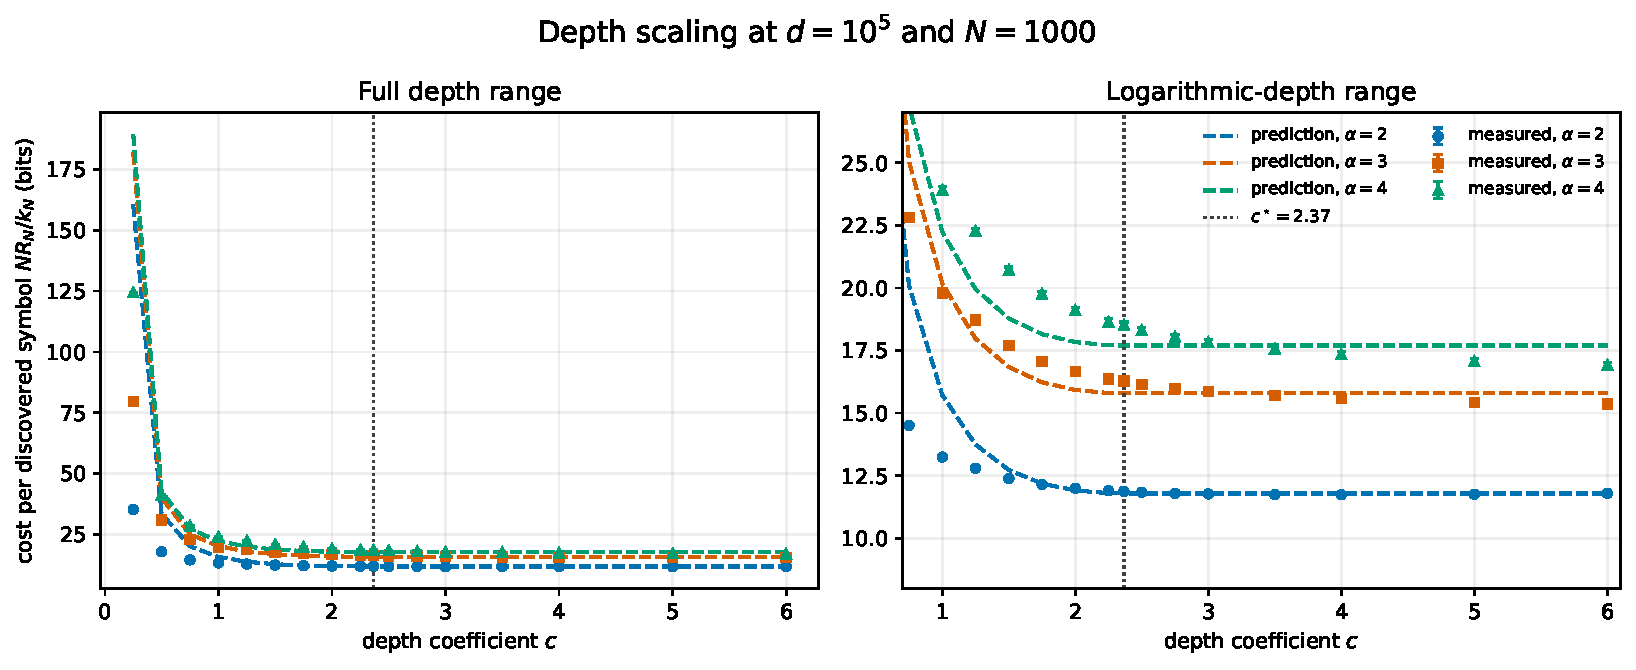
\includegraphics[width=0.78\textwidth]{figures/alt/depth_scaling.pdf}
\caption{Depth scaling. Regret per discovered symbol at $d=10^5$, $N=10^3$, with the modified single-weight heuristic described in the depth test (right: logarithmic-depth range enlarged). The heuristic captures the broad flattening at $\cstar$ and overestimates the shallowest depths.}
\label{fig:depth}
\end{figure*}

\paragraph{Benchmark estimators.} Here $c_t$ is the number of symbols appearing $t$ times, and $s$ is the number of observed symbols. \par\noindent\textbf{Add-one.} Laplace's rule. \par\noindent\textbf{Add-half.} The KT rule. \par\noindent\textbf{Good--Turing/empirical hybrid.} A symbol seen $t$ times receives (before normalization) the empirical mass $t/n$ if $t>c_{t+1}$ and the Good--Turing mass $(c_{t+1}+1)(t+1)/(nc_t)$ otherwise, each unseen symbol receiving the $t=0$ value. \par\noindent\textbf{Ristad's law.} The predictor is $\hat q(i)=(m_i+1)(n+1-s)/(n^2+n+2s)$ for $m_i>0$ and $s(s+1)/((d-s)(n^2+n+2s))$ for $m_i=0$ when $s<d$ (add-one if $s=d$). \par\noindent\textbf{Absolute discounting.} The predictor is $\hat q(i)=(m_i-\delta)/n$ for $m_i>0$ with $\delta=c_1/(c_1+2c_2)$. The discounted mass $\delta s/n$ is shared equally by the unseen symbols (if $c_1=0<c_2$, the discount is zero and the KL loss is infinite whenever unseen symbols have positive target probability; if $c_1=c_2=0$, the discount is undefined. These are the starred entries in Table~\ref{tab:bench}). \par\noindent\textbf{Dirichlet concentration mixture.} The exact evidence is $q_\tau(m)=\frac{\Gamma(\tau)}{\Gamma(\tau+n)}\prod_{i:m_i>0}\frac{\Gamma(m_i+\tau/d)}{\Gamma(\tau/d)}$. The component predictor is $(m_i+\tau/d)/(n+\tau)$. We use a uniform prior on the $29$-point grid $\tau/d=2^j$, $j=-24,\dots,4$, and posterior weights $\propto q_\tau(m)$. This mixture receives the same cumulative guarantee as Proposition~\ref{prop:avg}. \par\noindent\textbf{Natural oracle.} The predictor is $\hat q(i)=S_{m_i}/c_{m_i}$. It knows the target and must give equal probability to symbols with equal counts. \par\noindent\textbf{LSA.} The fixed-depth and depth-averaged predictors. \par 

\begin{table}[t]
\centering
\footnotesize
\caption{Mean posterior depth weights for the equal-prior mixture over $L=0,\ldots,80$. Broad posteriors are summarized by the shortest contiguous interval containing at least 95\% of the mean posterior mass (ties favor greater enclosed mass); the actual enclosed percentage is shown. Intervals spanning five or more depths are reported this way; otherwise individual weights of at least 0.05 are listed. Individual weights are rounded to two decimals.}
\label{tab:posteriors}
\setlength{\tabcolsep}{2pt}
\begin{tabular}{lll}
\toprule
target & posterior over depths at $n=10^3$ & at $n=2\cdot10^4$ \\
\midrule
uniform & $L{=}0:1.00$ & $L{=}0:1.00$ \\
step & $L{=}0:0.85$, $L{=}1:0.15$ & $L{=}0:1.00$ \\
Zipf $\alpha=1$ & $L{=}5:0.65$, $L{=}6:0.35$ & $L{=}3:1.00$ \\
Zipf $\alpha=1.5$ & broad: $97.2\%$ on $L\in[12,19]$ & $L{=}9:0.61$, $L{=}10:0.39$ \\
Zipf $\alpha=2$ & broad: $95.3\%$ on $L\in[19,53]$ & broad: $96.4\%$ on $L\in[20,31]$ \\
Zipf $\alpha=3$ & broad: $95.5\%$ on $L\in[40,80]$ & broad: $95.4\%$ on $L\in[46,80]$ \\
Zipf $\alpha=4$ & broad: $95.5\%$ on $L\in[42,80]$ & broad: $95.0\%$ on $L\in[52,80]$ \\
Zipf $\alpha=5$ & broad: $95.7\%$ on $L\in[42,80]$ & broad: $95.2\%$ on $L\in[53,80]$ \\
geometric & $L{=}4:0.76$, $L{=}5:0.24$ & $L{=}9:0.09$, $L{=}10:0.90$ \\
Dirichlet-1 & $L{=}1:1.00$ & $L{=}1:1.00$ \\
Dirichlet-$\frac12$ & $L{=}1:0.15$, $L{=}2:0.85$ & $L{=}2:1.00$ \\
\bottomrule
\end{tabular}
\end{table}

\paragraph{Bible controls and short prefixes.} A second tokenization of the Bible contains $917{,}868$ tokens and $13{,}554$ distinct types, with words and punctuation treated separately. The add-one, KT, Ristad, and GT control results on this tokenization agree with the values in Table~\ref{tab:bible} to within $0.001$ bits per token. The Dir-$\tau$ control uses the $29$-component mixture defined above. For short prefixes, the GT and LSA redundancies are respectively $3.066$ and $3.071$ at $n=500$, and $3.747$ and $3.826$ at $n=100$, in bits per token.

\end{document}
